\documentclass[12pt]{book}

\usepackage{mathptm,times,color}
\usepackage[pdftex]{graphicx}
\usepackage{multirow}
\usepackage{bezier}
\usepackage{rotating}
\usepackage{longtable}
\usepackage{amsmath}
\usepackage{xfrac}
\usepackage{array}
\usepackage{units}
\usepackage{fix-cm}
\usepackage{makeidx} % Create index at end of document
\usepackage[nottoc,notlof,notlot]{tocbibind} % Put the bibliography and index in the ToC
\usepackage{datetime}
\newdateformat{mydate}{\monthname[\THEMONTH] \THEYEAR}

\usepackage{listings}
\usepackage{textcomp}
\definecolor{lbcolor}{rgb}{0.96,0.96,0.96}
\lstset{
    %backgroundcolor=\color{lbcolor},
    tabsize=4,
    rulecolor=,
    language=Fortran,
        basicstyle=\footnotesize\ttfamily,
        upquote=true,
        aboveskip={\baselineskip},
        belowskip={\baselineskip},
        columns=fixed,
        extendedchars=true,
        breaklines=true,
        breakatwhitespace=true,
        frame=none,
        showtabs=false,
        showspaces=false,
        showstringspaces=false,
        identifierstyle=\ttfamily,
        keywordstyle=\color[rgb]{0,0,0},
        commentstyle=\color[rgb]{0,0,0},
        stringstyle=\color[rgb]{0,0,0},
}

\usepackage{wrapfig}

\newcolumntype{L}[1]{>{\raggedright\let\newline\\\arraybackslash\hspace{0pt}}m{#1}}
\newcolumntype{C}[1]{>{\centering\let\newline\\\arraybackslash\hspace{0pt}}m{#1}}
\newcolumntype{R}[1]{>{\raggedleft\let\newline\\\arraybackslash\hspace{0pt}}m{#1}}

\usepackage{framed}
\newcommand{\graybox}[1]{
\begin{shaded}#1\end{shaded}
}

\renewcommand{\bibname}{References}

% dummy change to force revision update

%\usepackage{eso-pic}
%\usepackage{graphicx}
%\usepackage{color}
%\usepackage{type1cm}


%\makeatletter
%   \AddToShipoutPicture{%
%     \setlength{\@tempdimb}{.5\paperwidth}%
%    \setlength{\@tempdimc}{.5\paperheight}%
%   \setlength{\unitlength}{1pt}%
%  \put(\strip@pt\@tempdimb,\strip@pt\@tempdimc){%
%     \makebox(0,0){\rotatebox{45}{\textcolor[gray]{0.75}{\fontsize{8cm}{8cm}\selectfont{DRAFT}}}}}}
%\makeatother

\definecolor{linknavy}{rgb}{0,0,0.50196}
\definecolor{linkred}{rgb}{1,0,0}
\definecolor{linkblue}{rgb}{0,0,1}
\definecolor{shadecolor}{rgb}{0.9,0.9,0.9}

\usepackage[pdftex,
        colorlinks=true,
        urlcolor=linkblue,     % \href{...}{...} external (URL)
        citecolor=linkred,     % citation number colors
        linkcolor=linknavy,    % \ref{...} and \pageref{...}
        pdfproducer={pdflatex},
        pagebackref,
        pdfpagemode=UseNone,
        bookmarksopen=true,
        plainpages=false,
        verbose]{hyperref}

% CFAST Version String
\newcommand{\cfastversion}{7.0.0}

% commands to use for "official" cover and title pages
% see smokeview verification guide to see how they are used

\newcommand{\logosigs}{
\begin{minipage}[b]{6.5in}
\flushright{
\includegraphics[height=1.05in]{FIGURES/nistident}}
\end{minipage}
}

\newcommand{\titlesigs}
{
\small
\begin{flushright}
U.S. Department of Commerce \\
{\em Penny Pritzker, Secretary} \\
\hspace{1in} \\
National Institute of Standards and Technology \\
{\em Willie May, Acting Under Secretary of Commerce for Standards and Technology and Acting Director}
\end{flushright}
}

\newcommand{\headerA}[1]{
\begin{flushright}
\fontsize{20}{24}\selectfont
\bf{NIST Technical Note #1}
\end{flushright}
}


\newcommand{\headerB}[1]{
\begin{flushright}
\fontsize{28}{33.6}\selectfont
\bf{#1}
\end{flushright}
}

\newcommand{\headerC}[1]{
\vspace{.15in}
\begin{flushright}
\fontsize{12}{14}\selectfont
#1
\end{flushright}
}

\newcommand{\headerD}[1]{
\begin{flushright}
\fontsize{12}{14}\selectfont
This publication is available free of charge from: \\
http://dx.doi.org/10.6028/NIST.TN.#1
\end{flushright}
}



\setlength{\textwidth}{6.5in}
\setlength{\textheight}{9.0in}
\setlength{\topmargin}{0.in}
\setlength{\headheight}{0.in}
\setlength{\headsep}{0.in}
\setlength{\parindent}{0.25in}
\setlength{\oddsidemargin}{0.0in}
\setlength{\evensidemargin}{0.0in}


\newcommand{\brackets}[1]{ { \left( {#1} \right) } }
\newcommand{\dbydt}[1]{\frac{d {#1}}{dt}}
\newcommand{\superscript}[1]{\ensuremath{^{\textnormal{\scriptsize \hbox{#1}}}}}
\newcommand{\subscript}[1]{\ensuremath{_{\textnormal{\scriptsize \hbox{#1}}}}}

\newcommand{\trho}{\tilde{\rho}}
\newcommand{\dph}{{\delta\phi}}
\newcommand{\dth}{{\delta\theta}}
\newcommand{\tp}{\tilde{p}}
\newcommand{\dQ}{\dot{Q}}
\newcommand{\dQc}{\dot{Q}_{\rm c}}
\newcommand{\dQr}{\dot{Q}_{\rm r}}
\newcommand{\Dh}{\Delta h}
\newcommand{\DhO}{\Delta h_\OTWO}
\newcommand{\Tp}{T_{\rm p}}
\newcommand{\Tu}{T_{\rm u}}
\newcommand{\Tl}{T_{\rm l}}
\newcommand{\Ts}{T_{\rm s}}
\newcommand{\Tg}{T_{\rm g}}
\newcommand{\TL}{T_{\rm L}}
\newcommand{\Vu}{V_{\rm u}}
\newcommand{\Vl}{V_{\rm l}}
\newcommand{\doh}{\dot{h}}
\newcommand{\dhl}{\dot{h}_{\rm l}}
\newcommand{\dhu}{\dot{h}_{\rm u}}
\newcommand{\dmal}{\dot{m}_{\rm l}}
\newcommand{\dmau}{\dot{m}_{\rm u}}
\newcommand{\dq}{\dot{q}}
\newcommand{\dqc}{\dot{q}_{\rm c}}
\newcommand{\dqr}{\dot{q}_{\rm r}}
\newcommand{\dm}{\dot{m}}
\newcommand{\dme}{\dot{m}_{\rm e}}
\newcommand{\dmp}{\dot{m}_{\rm p}}
\newcommand{\dml}{\dot{m}_{\rm l}}
\newcommand{\dmu}{\dot{m}_{\rm u}}
\newcommand{\dmf}{\dot{m}_{\rm f}}

\newcommand{\be}{\begin{equation}}
\newcommand{\ee}{\end{equation}}

\newcommand{\RE}{\hbox{Re}}
\newcommand{\LE}{\hbox{Le}}
\newcommand{\PR}{\hbox{Pr}}
\newcommand{\PE}{\hbox{Pe}}
\newcommand{\NU}{\hbox{Nu}}
\newcommand{\SC}{\hbox{Sc}}
\newcommand{\SH}{\hbox{Sh}}
\newcommand{\WE}{\hbox{We}}

\newcommand{\COTWO}{{\tiny \hbox{CO}_2}}
\newcommand{\OTWO}{{\tiny \hbox{O}_2}}
\newcommand{\CO}{{\tiny \hbox{CO}}}
\newcommand{\HTWOO}{{\tiny \hbox{H}_2\hbox{O}}}
\newcommand{\NTWO}{{\tiny \hbox{N}_2}}
\newcommand{\F}{{\tiny \hbox{F}}}
\newcommand{\So}{{\tiny \hbox{S}}}
\newcommand{\M}{{\tiny \hbox{M}}}
\newcommand{\HCN}{{\tiny \hbox{HCN}}}
\newcommand{\HCl}{{\tiny \hbox{HCl}}}
\newcommand{\Hy}{{\tiny \hbox{H}}}
\newcommand{\C}{{\tiny \hbox{C}}}
\newcommand{\N}{{\tiny \hbox{N}}}
\newcommand{\Oh}{{\tiny \hbox{O}}}
\newcommand{\Cl}{{\tiny \hbox{Cl}}}

\newcommand{\asqh}{$A_T/A\sqrt{h}$}
\newcommand{\degc}{$^{\circ}$C }
\newcommand{\degf}{$^{\circ}$F }

\newcommand{\dx}{\delta x}
\newcommand{\dy}{\delta y}
\newcommand{\dz}{\delta z}
\newcommand{\dt}{\delta t}

\newcommand{\ha}{\frac{1}{2}}
\newcommand{\ft}{\frac{4}{3}}
\newcommand{\ot}{\frac{1}{3}}
\newcommand{\fofi}{\frac{4}{5}}
\newcommand{\of}{\frac{1}{4}}
\newcommand{\twth}{\frac{2}{3}}


\newcommand{\rb}[1]{\raisebox{1.5ex}[0pt]{#1}}

\newcommand{\erf}{\hbox{erf}}



\begin{document}

\bibliographystyle{unsrt}

\frontmatter

\pagestyle{empty}


\begin{minipage}[t][9in][s]{6.5in}

\headerA{XXXX\\}

\headerB{
CFAST -- Consolidated Model of Fire \\
 Growth and Smoke Transport \\
 (Version 7) \\
 Volume 2: User's Guide \\
}

\headerC{
   Richard D. Peacock \\
   Paul A. Reneke \\
   Glenn P. Forney \\
}

\vfill

\headerD{XXXXv2}

\vfill

\logosigs

\end{minipage}

\newpage

\hspace{5in}

\newpage

\begin{minipage}[t][9in][s]{6.5in}

\headerA{XXXX\\}

\headerB{
CFAST -- Consolidated Model of Fire \\
 Growth and Smoke Transport \\
 (Version 7) \\
 Volume 2: User's Guide \\
}

\headerC{
   Richard D. Peacock \\
   Paul A. Reneke \\
   Glenn P. Forney \\
}

\headerD{XXXXv2}

\headerC{
\flushright{\mydate\today\\
CFAST Version \cfastversion \\
\emph{SVN Repository}~$Revision$}}
% dummy comment to force svn change - Mon Jan  5 21:57:14 EST 2015

\vfill

\flushright{
\includegraphics[width=1.2in]{FIGURES/doc} }

\titlesigs

\end{minipage}


\newpage

\frontmatter

\pagestyle{plain}
\setcounter{page}{3}

\chapter{Disclaimer}

The U. S. Department of Commerce makes no warranty, expressed or implied, to users of
CFAST and associated computer programs, and accepts no responsibility for its use.  Users of
CFAST assume sole responsibility under Federal law for determining the appropriateness of its
use in any particular application; for any conclusions drawn from the results of its use; and for
any actions taken or not taken as a result of analyses performed using these tools.
CFAST is intended for use only by those competent in the field of fire safety and is intended
only to supplement the informed judgment of a qualified user. The software package is a
computer model which may or may not have predictive value when applied to a specific set of
factual circumstances. Lack of accurate predictions by the model could lead to erroneous
conclusions with regard to fire safety. All results should be evaluated by an informed user.

\chapter{Intent and Use}

The algorithms, procedures, and computer programs described in this report constitute a
methodology for predicting some of the consequences resulting from a prescribed fire.  They
have been compiled from the best knowledge and understanding currently available, but have
important limitations that must be understood and considered by the user.  The program is
intended for use by persons competent in the field of fire safety and with some familiarity with
personal computers. It is intended as an aid in the fire safety decision-making process.

\chapter{Abstract}

CFAST is a two-zone fire model capable of predicting the environment in a multi-compartment structure subjected to a fire. It calculates the time-evolving distribution of smoke and gaseous combustion products as well as the temperature throughout a building during a user-prescribed fire. This report describes the use of the model, including installing and running the software, the computer platforms upon which it is supported and examples to verify correct installation.

\chapter{Acknowledgments}

\label{acksection}

Continuing support for CFAST is via internal funding at NIST. In addition, support is provided by other agencies of the U.S. Federal Government, most notably the Nuclear Regulatory Commission Office of Nuclear Regulatory Research and the U.S. Department of Energy. The U.S. NRC Office of Nuclear Regulatory Research has funded key validation experiments, the preparation of the CFAST manuals, and the continuing development of sub-models that are of importance in the area of nuclear power plant safety. Special thanks to Mark Salley and David Stroup for their efforts and support.

Support to refine the software development and quality assurance process for CFAST has been provided by the U.S. Department of Energy (DOE). The assistance of Subir Sen and Debra Sparkman in understanding DOE software quality assurance programs and the application of the process to CFAST is gratefully acknowledged. Thanks are also due to Allan Coutts, Washington Safety Management Solutions for his insight into the application of fire models to nuclear safety applications and detailed review of the CFAST document updates for DOE.

\tableofcontents

\listoffigures

\mainmatter


\chapter{Getting Started}

\section{Installation from the CFAST Web Site}

CFAST is documented by three publications, this user's guide, a technical reference guide \cite{CFAST_Tech_Guide_7} and a model evaluation guide \cite{CFAST_Valid_Guide_7}. The technical reference guide describes the underlying physical principles, provides a comparison with other models, and includes an evaluation of the model following the guidelines of ASTM E1355 \cite{ASTM:E1355}. The model evaluation guide documents verification and validation efforts for the model. This user's guide describes how to use the model and applies to version 67 and later.  All the documentation is available on the web site.

All of the files associated with CFAST can be obtained at:

\begin{lstlisting}
http://cfast.nist.gov
\end{lstlisting}

\begin{wrapfigure}{r}{3.2in}
  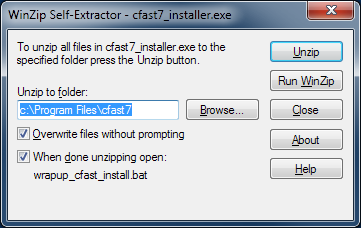
\includegraphics[width=3.1in]{FIGURES/Getting_Started/Install}
\end{wrapfigure}

Information about new versions, bug fixes, and documentation for the model and software are available on this web site.  The CFAST distribution consists of a self-extracting set-up program for Windows-based PCs.

After downloading the set-up program to a PC, double-clicking on the file's icon walks the user through a series of steps for installation of the program.  The most important part of the installation is the creation of a folder (typically c:$\backslash$Program Files$\backslash$CFAST by default) in which the CFAST executable files and supplemental data files are installed.  Sample input files are placed in a folder called Examples off this folder.

\section{Computer Hardware Requirements}
CFAST requires a relatively fast processor and a sufficient amount of random-access memory (RAM) for complex cases. Typical calculation times for a multi-compartment scenario can range from a few seconds to multiple hours, depending on the details of the scenario. Plus, hard drive storage is needed to store the output of calculations.  It is not uncommon for a single calculation to generate output files as large as several hundred megabytes.

\section{Verifying Correct Installation and Operation}
Sample input files are provided with the program for new users who are encouraged to first run the sample calculations before attempting to create an input file. To run the model, browse to the location of the CFAST sample input file (default location is in a folder called Examples off the installation folder, copy the file named standard.in to a location of your choice (for example, in a created folder of the ``My Documents'' folder and then double click on the copied file.  This should open the file in the CFAST input editor, CEdit.  The simple test case can be run from the program menu by selecting 'Run!' and then 'Model Simulation, CFAST'

This runs a very simple test case and it should be completed quickly. Additional details on running CFAST are included in the next chapter. To verify that the installation has been done correctly, the output of the model should appear as follows.

\begin{figure}[h!]
\begin{center}
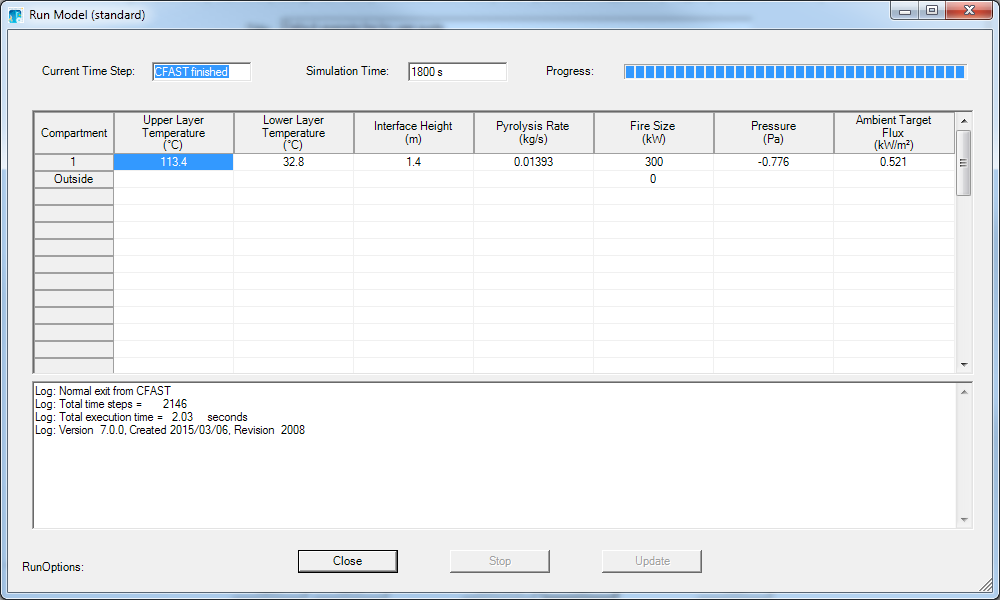
\includegraphics[width=6.5in]{FIGURES/Getting_Started/Standard_Output}
\end{center}
\end{figure}

This case checks several attributes of the installation to insure the software is running correctly. Additional explanation of the results of this run is described in Chapter 5.

\chapter{Setting Up the Input File for CFAST}

\section{Overview}

CFAST is a computer program that uses an input file and generates one or more output files. The first step in performing a calculation is to generate a text input file that provides the program with all of the necessary information to describe the scenario under consideration.  The most important inputs determine the geometry of the compartments in the scenario and the connections between these compartments. Next, the fire, detection, and suppression characteristics of the scenario are defined. Finally, there are a number of parameters that customize the output from the model.  Each line of the file contains a keyword label that identifies the input, followed by a number of numerical or text inputs corresponding to the particular input keyword. A simple input file is shown below. This example is used in the discussion of the output in Chapter 5.

\begin{lstlisting}
VERSN,6,Cable tray fire -- base case
!!
!!Scenario Configuration Keywords
!!
TIMES,1800,-120,10,30
EAMB,293.15,101300,0
TAMB,293.15,101300,0,50
CJET,WALLS
WIND,0,10,0.16
!!
!!Material Properties
!!
MATL,CONCRETE,1.75,1000,2200,0.15,0.94,"Concrete, Normal Weight (6 in)"
MATL,GLASSFB3,0.036,795,105,0.013,0.9,"Glass Fiber, Organic Bonded (1/2 in)"
MATL,METHANE,0.07,1090,930,0.0127,0.04,"Methane, a transparent gas (CH4)"
MATL,HARDWOOD,0.16,1255,720,0.019,0.9,"Wood, Hardwoods (oak, maple) (3/4 in)"
!!
!!Compartment keywords
!!
COMPA,Compartment 1,9.1,5,4.6,0,0,0,GLASSFB3,CONCRETE,CONCRETE
!!
!!Vent keywords
!!
HVENT,1,2,1,1,2.4,0,1,0,0,1,1
!!
!!Fire keywords
!!
GLOBA,10,393.15
!!Wood_Wall
FIRE,1,4.55,2.5,0,1,1,0,0,0,1,Wood_Wall
CHEMI,1,4,0,0,0,0.33,1.81E+07,HARDWOOD
TIME,0,8000
HRR,0,1000000
SOOT,0.02,0.02
CO,0.02,0.02
TRACE,0,0
AREA,0.05,9
HEIGH,0,3
!!
!!Target and detector keywords
!!
TARGET,1,2.2,1.88,2.34,0,0,1,CONCRETE,IMPLICIT,PDE,0.5
\end{lstlisting}

All of the inputs to the model are discussed in this chapter.  Following the discussion that details each input, their engineering units and default values, notes are included that provided additional guidance or frequently addressed problems that may be encountered by the user. These notes take the form of a bulleted list such as:

\begin{itemize}
\item The inputs may be integers (e.g., a simulation time of 1800 s), real numbers (a mass loss rate of 0.0082 kg/s), or text (a floor material of CONCRETE), as appropriate. The input file is a comma-separated ASCII text file and may be edited with a spreadsheet program or any text editor. It is possible to use a word processor but it is important to save the file in ASCII text format and not in a word processing format. Note that some word processors will save punctuation and other characters incorrectly for the simple ASCII text file used by CFAST. It is recommended that the input files be created with the input editor, CEdit, provided as part of the CFAST distribution.  In addition to checking the input data for errors, it includes typical ranges for input values to assist in appropriate use of the model.

\item Numeric format for inputs to CFAST and the input editor CEdit assume a period is used to separate the integer and fractional parts of the number. No separator is used to group digits in the integer part of numbers.

\item Each line of input consists of a label followed by one or more alphanumeric parameters associated with that input label, separated by commas.  The label must always begin in the first space of the line and be in capital letters.  Following the label, the values may start in any column, and all values must be separated by a comma.  Values may contain decimal points if needed or desired.  They are not required.  

\item Inputs are in standard SI units.  The maximum line length is 1024 characters, so all data for each keyword must fit in this number of characters.
\end{itemize}

The installation program creates a shortcut to the input editor on the Windows start menu labeled "CFAST" that points to the input editor.  Once started, the user is presented with a series of tabbed-pages for the various inputs in a CFAST input data file.

\begin{figure}[h!]
\begin{center}
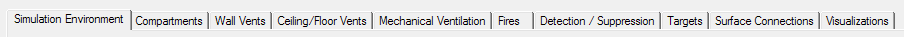
\includegraphics[width=6.5in]{FIGURES/Input_File/Tabs}
\end{center}
\end{figure}

These tabbed-pages organize the inputs for CFAST simulations into several categories as follows.
\begin{itemize}
\item \textbf{Simulation Environment} includes simulation time, specification of model outputs, and ambient conditions. Also included on the page are a constantly updated list of errors, warnings, and messages about the input file specification or model simulation.
\item \textbf{Compartment Geometry} defines the size, construction characteristics, and position of the compartments in a simulation.
\item \textbf{Wall Vents, Ceiling/Floor Vents, and Mechanical Flow Vents} allows the user to connect compartments with doors and windows, ceiling and floor vents, or forced air ventilation systems.
\item \textbf{Fires} include user specification of the initial fire source and any additional burning objects in one or more of the compartments of the simulation.
\item \textbf{Detection / Suppression}defines any heat alarms and sprinklers in the compartments of the simulation.
\item \textbf{Targets} provide the ability calculate the temperature and net heat flux to objects placed and oriented arbitrarily in the structure.
\item \textbf{Surface Connections} allows for more detailed description of the connections between compartments in the simulation to better simulate the transfer of heat from compartment to compartment in the simulation.
\end{itemize}

Each of these tabbed-pages is described in more detail below. In addition, a series of menus allow the user to open and save files; run the simulation, or access help and program information.

\section{Simulation Environment}

The Simulation Environment page defines the initial conditions and simulation time for the CFAST input file. 

\begin{figure}[h!]
\begin{center}
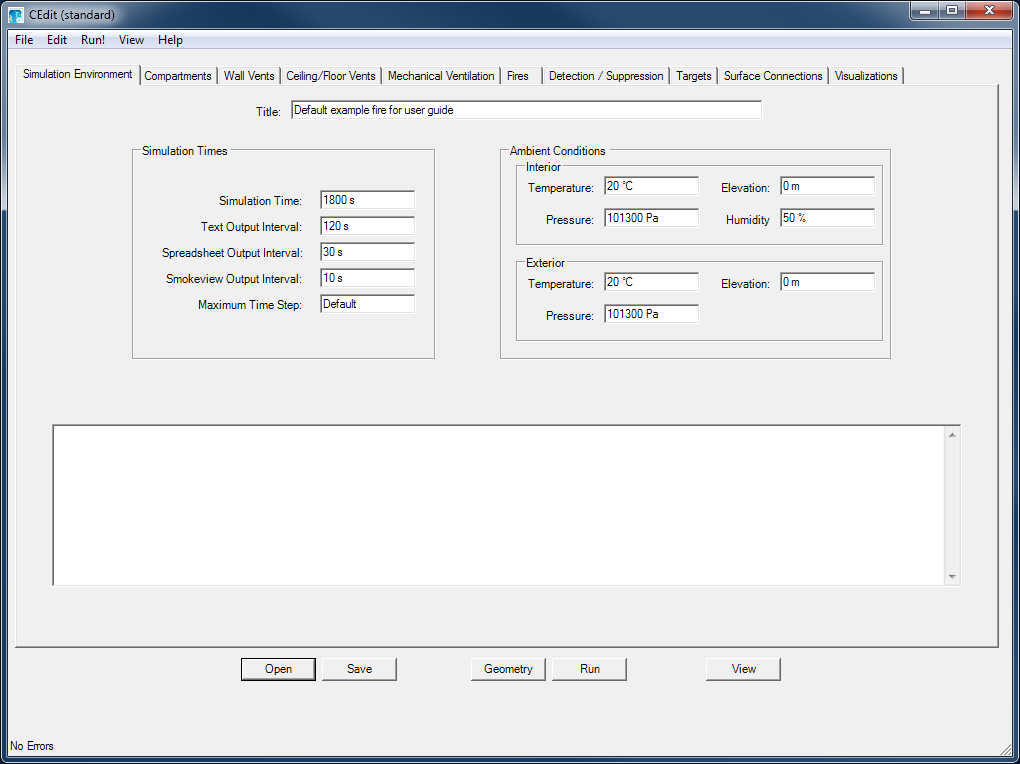
\includegraphics[width=6.5in]{FIGURES/Input_File/Environment_Tab}
\end{center}
\end{figure}

\subsection{Naming the Calculation, the Title Input}

The first thing to do when setting up an input file is to give the simulation a title.  The first line in the CFAST input data file must be the CFAST version identification along with an optional short title for the simulation.  This is a required input.  The title command is the line that CFAST keys on to determine whether it has a correct data file.

\begin{lstlisting}
VERSN,6,CFAST Simulation
\end{lstlisting}

\clearpage

\begin{figure}[h!]
\begin{center}

\includegraphics[width=3.458in]{FIGURES/Input_File/Title}
\end{center}
\end{figure}

\textbf{Title:} The title is optional and may consist of letters, numbers, and/or symbols and may be up to 50 characters. It permits the user to label each run.

\subsection{Setting Time Limits and Output Options}

A TIMES line specifies the length of time over which the simulation takes place and how often output will be generated. This is a required input. There are one to four entries in this line.

\begin{lstlisting}
TIMES,900,50,10,10
\end{lstlisting}

\begin{figure}[h!]
\begin{center}
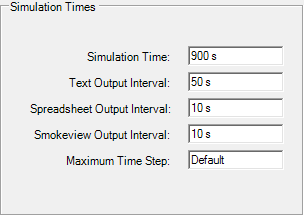
\includegraphics[width=3.167in]{FIGURES/Input_File/Simulation_Times}
\end{center}
\end{figure}

\begin{itemize}
\item \textbf{Simulation Time} (default units: s, default value, 900 s): The length of time over which the simulation takes place.  This is a required input which should be entered even if all other fields are not included. The maximum value for this input is 86400 s (1 day).

\item \textbf{Text Output Interval} (default units: s, default value, 50 s): The print interval is the time interval between each printing of the output values.  If omitted or less than or equal to zero, no output values will occur.

\item \textbf{Spreadsheet Output Interval} (default units: s, default value, 10 s): CFAST can output a subset of the results of the model simulation in a comma-delimited alphanumeric format which can be read by most spreadsheet software. This is designed to be imported into a spreadsheet for further analysis or graphing of the results of the simulation.  This input defines the time interval between outputs of the model results in a spreadsheet-compatible format. A value greater than zero must be used if the spreadsheet file is to be used.

\item \textbf{Smokeview Output Interval} (default units: s, default value: 10 s): CFAST can output a subset of the results in a format compatible with the visualization program smokeview. This input defines the time interval between outputs of the model results in a smokeview-compatible format.  A value greater than zero must be used if the spreadsheet output is desired.
\end{itemize}

In addition to the input data file created specifically for a CFAST simulation, there are a number files that CFAST uses to define default values and other input information, and to output the results of the simulation for later analysis.  They include 1) a thermal properties file, 2) files of predefined fire objects, and 4) a spreadsheet-compatible output file.

The thermal properties file contains material properties for compartment surfaces, target objects that may be placed in compartments in the simulation to monitor surface temperature and heat flux to the objects, and fire objects, in addition to the main fire in the simulation that may ignite based on their surface temperature or incident flux onto the surface of the object. The predefined fire objects files contain definitions for a number of reference fires from the literature or developed by the user that may be included in a simulation. The thermal properties and fire objects files may be modified by the user.  Details of the files are included in the appendices.  There are default files included in the CFAST distribution.

\subsection{Ambient Conditions}

Ambient conditions define the environment at which the scenario begins. This allows the user to specify the temperature, pressure, and station elevation of the ambient atmosphere, as well as the absolute wind pressure to which the structure is subjected.  Pressure interior to a structure is calculated simply as a lapse rate (related to the height above sea level) based on the NOAA/NASA tables \cite{GPO:Atmosphere}.  This modification is applied to the vents which connect to the exterior ambient.  The calculated pressure change is modified by the wind coefficient for each vent.  This coefficient, which can vary from -1.0 to +1.0, nominally from -0.8 to +0.8, determines whether the vent is facing away from or into the wind.  The pressure change is multiplied by the vent wind coefficient and added to the external ambient for each vent which is connected to the outside. There is an ambient for the interior and for the exterior of the structure.  Three keywords define the ambient conditions: TAMB for the interior of the structure, EAMB for the exterior of the structure is EAMB, and WIND for the wind information.

\begin{lstlisting}
EAMB,293.15,101300,0
TAMB,293.15,101300,0,50
WIND,0,10,0.16
\end{lstlisting}

\begin{figure}[h!]
\begin{center}
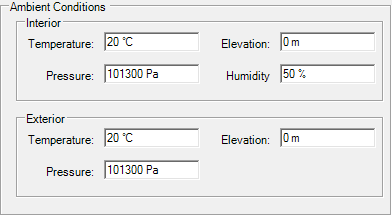
\includegraphics[width=4.313in]{FIGURES/Input_File/Ambient_Conditions}
\end{center}
\end{figure}

\textbf{Ambient Temperature} (default units: \degc~C, default value: 20 \degc~C): Initial ambient temperature inside (for TAMB) or outside (For EAMB) the structure at the station elevation.

\textbf{Ambient Pressure} (default units: Pa, default value: 101300 Pa): Initial values for ambient atmospheric pressure inside (for TAMB) and outside (for EAMB) the structure at the station elevation. Default value is standard atmospheric pressure at sea level (0 m elevation) of 101.3 kPa. Input units are in Pa. These values define standard conditions as defined in Standard Atmosphere as noted in the Handbook of Chemistry and Physics  . There is a set of numerical approximations in the CFAST code which duplicate the pressure/temperature/altitude relationships in the handbook.

\textbf{Elevation} (defaults units: m, default value: 0 m): The height where the ambient pressure and temperature were specified.  This is the reference datum for calculating the density of the atmosphere as well as the temperature and pressure inside and outside of the structure as a function of height.  

\textbf{Relative Humidity} (default units \% RH, default value: 50 \%): The initial relative humidity in the system, only specified for the interior with the TAMB command.  This is converted to kilograms of water per cubic meter.

The wind speed, scale height, and power law are used to calculate the wind coefficient for each vent connected to the outside.  The wind velocity is specified at some reference height.  The power law then provides a lapse rate for the wind speed.  An assumption is that the wind speed is zero at the surface.  The formula used to calculate the wind speed at the height of any vent is show below.  The wind is applied to each external opening as a change in pressure outside of the vent.

\textbf{Wind Speed} (default units: m/s, default value 0 m/s): Wind speed at the reference elevation.

\textbf{Scale Height} (default units: m, default value: 0 m)): Reference height at which the reference wind speed is measured.

\textbf{Power Law Coefficient} (default units: dimensionless, default value 0.16): The power law used to calculate the wind speed as a function of height. Default value is 0.16. Using the notation that $V_W$, is the wind speed at the reference height $H_W$, and $P_W$ is the power law, the exterior pressure is modified by  $\delta P = {C_W}{V^2}$ and $V = {V_W}{\left( {\frac{{{H_i}}}{{{H_W}}}} \right)^{{P_W}}}$ where $H_i$ is the position of the vent \cite{CFAST_Tech_Guide_6}.

\begin{itemize}
\item In order to see the effect of wind, the corresponding parameter for the ventilation keyword must be specified. The default for the wind vector is 0, which turns off wind effects. Please see the HVENT command, below.

\item The choice for station elevation, temperature and pressure must be consistent.  Outside of that limitation, the choice is arbitrary.  It is often convenient to choose the base of a structure to be at zero height and then reference the height of the structure with respect to that height.  The temperature and pressure must then be measured at that position.  Another possible choice would be the pressure and temperature at sea level, with the structure elevations then given with respect to mean sea level.  This is also acceptable, but somewhat more tedious in specifying the construction of a structure.  Either of these choices works though, so long as they are consistent. Usually, the station elevation is set to zero and the pressure to ambient. The effect of changing these values is small for small changes. There will be an effect for places at altitude such as Denver, Colorado, but even there the effect is not pronounced. Note that the equations implemented in the model are not designed to handle negative elevations and altitudes. It is suggested that the defaults be used.

\item These three parameters are optional. If they are not included in the input file, default values are used.
\end{itemize}

\section{Compartment Geometry}

The Compartment Geometry page defines the size, position, materials of construction, and flow characteristics for the compartments in the simulation. Initially, only the simulation environment page and the �Add� button on the compartment geometry page is enabled; all other pages are not available to the user for detailed inputs until a compartment has been added to the simulation.  

\begin{figure}[h!]
\begin{center}
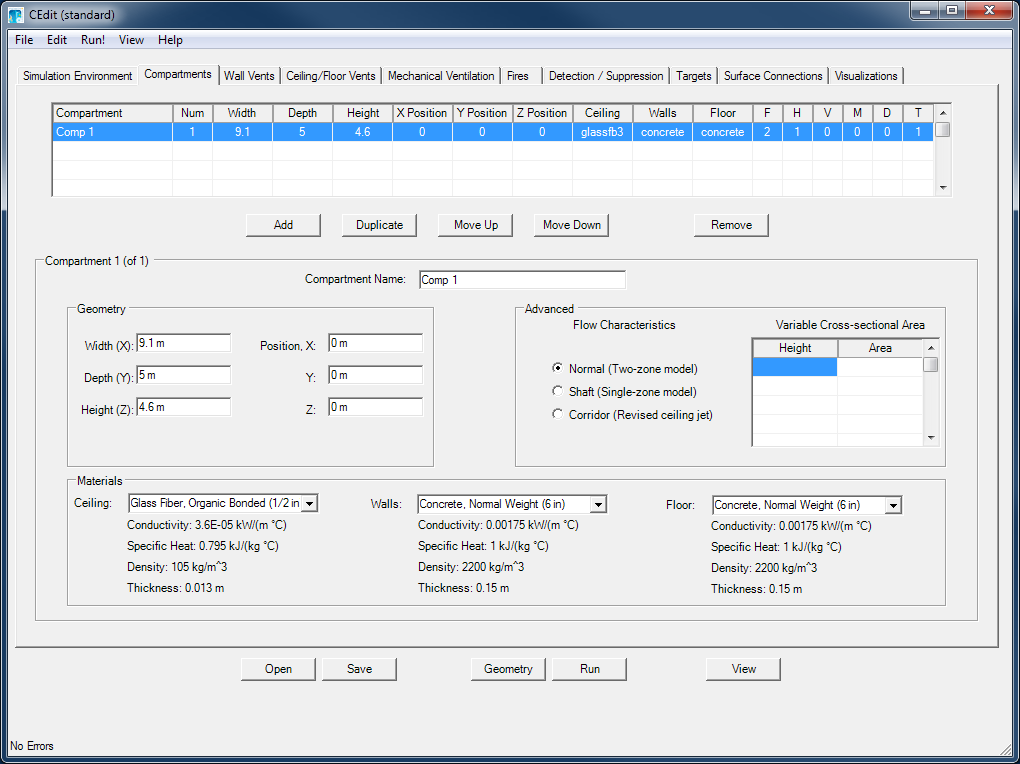
\includegraphics[width=6.5in]{FIGURES/Input_File/Compartment_Geometry_Tab}
\end{center}
\end{figure}

Most of the tabbed pages in the program are of similar design, with a summary of the defined items in table form at the top of the page, a series of buttons to add, remove, or modify the item highlighted in the summary table, and a number of individual inputs below which details all of the inputs for the item selected in the summary table. The buttons included on the compartment geometry page are as follows: \\

\begin{wrapfigure}{l}{0pt}
  
\includegraphics[width=0.781in]{FIGURES/Input_File/Add_Button}
\end{wrapfigure}

Use the Add button to create a new compartment with default values for all entries. \\~ \\

\begin{wrapfigure}{l}{0pt}
  
\includegraphics[width=0.781in]{FIGURES/Input_File/Duplicate_Button}
\end{wrapfigure}

Use the Duplicate button to create a copy of the compartment currently selected in the summary table at the top of the page. The new compartment is added to the end of the list with the named changed to indicate it is a copy of the selected item. \\

\begin{wrapfigure}{l}{0pt}
  
\includegraphics[width=0.781in]{FIGURES/Input_File/Move_Up_Button}
\end{wrapfigure}

Use the Move Up and Move Down buttons to change the order of the list of compartments in the summary table. This simply changes the automatically assigned compartment numbers for the compartments. Compartments can be ordered as desired.

\begin{wrapfigure}{l}{0pt}
  
\includegraphics[width=0.781in]{FIGURES/Input_File/Remove_Button}
\end{wrapfigure}

Use the Remove button to delete the selected compartment from the list of compartments in the summary table.  Other compartments are renumbered once the compartment is deleted.

\subsection{Defining the Compartment}

In order to model a fire scenario, the size and elevation of each compartment in the structure must be specified. For a compartment, the width, depth, compartment height and height of the floor of the compartment provide this specification. The maximum number of compartments for version 6 is thirty. The usual assumption is that compartments are rectangular parallelepipeds. However, the CFAST model can accommodate odd shapes as equivalent floor area parallelepipeds or with a cross-sectional area that varies with height.

At least one compartment must be specified in the input file.  There are no defaults for compartment size. There are defaults for absolute positioning (0,0,0). The fully mixed (single zone) and corridor models are turned off by default.

\begin{wrapfigure}{r}{0pt}
  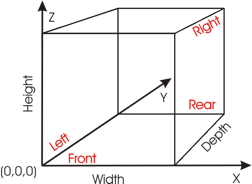
\includegraphics[width=2.0in]{FIGURES/Input_File/CFAST_Coordinates}
\end{wrapfigure}

Compartments in CFAST are most typically defined by a width, depth, and height.  If desired, compartments can be prescribed by the cross-sectional area of the compartment as a function of height from floor to ceiling for other shapes. The absolute position of the compartment with respect to a single structure reference point can be defined to ease visualization or to allow exact placement of vents and surfaces relative to other compartments in a detailed calculation. This specification is important for utilizing the corridor flow algorithm with the HALL command and for positioning the compartments for visualization in SMOKEVIEW. 

The relevant CFAST keywords are COMPA to define the compartment size and materials, HALL or ONEZ to define flow characteristics in the compartment, and ROOMA / ROOMH to define a variable cross-sectional area for the compartment. The COMPA command is required for each compartment as a basic definition for the compartment, even if there are subsequent modifications by the HALL, ONEZ, ROOMA, or ROOMH keywords which follow.  Details of the CFAST keywords are included in Appendix A.

\begin{lstlisting}
COMPA,Compartment 1,9.1,5,4.6,0,0,0,GLASSFB3,CONCRETE,CONCRETE
\end{lstlisting}

\begin{figure}[h!]
\begin{center}

\includegraphics[width=4.0in]{FIGURES/Input_File/Compartment_Name}
\end{center}
\end{figure}

\textbf{Compartment Name:} Compartments are identified by a unique alphanumeric name.  This may be a simple as a single character or number, or a description of the compartment.

\begin{figure}[h!]
\begin{center}
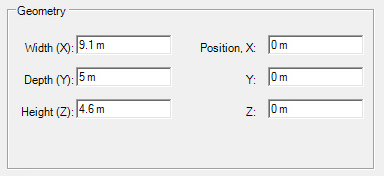
\includegraphics[width=3.552in]{FIGURES/Input_File/Compartment_Size}
\end{center}
\end{figure}

\textbf{Width:} specifies the width of the compartment as measured on the X axis from the origin (0,0,0) of the compartment.  

\textbf{Depth:} specifies the depth of the compartment as measured on the Y axis from the origin (0,0,0) of the compartment.  

\textbf{Height:} specifies the height of the compartment as measured on the Z axis from the origin (0,0,0) of the compartment.  

\begin{wrapfigure}{r}{0pt}
  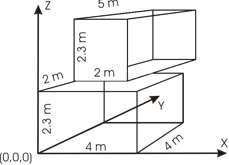
\includegraphics[width=2.0in]{FIGURES/Input_File/CFAST_Absolute_Positioning}
\end{wrapfigure}

\textbf{Absolute Width Position:} specifies the absolute x coordinate of the lower, left, front corner of the room.

\textbf{Absolute Depth Position:} specifies the absolute y coordinate of the lower, left, front corner of the room.

\textbf{Absolute Floor Height:} specifies the height of the floor of each compartment with respect to station elevation specified by the internal ambient conditions reference height parameter.  The reference point must be the same for all elevations in the input data.  For example, the two rooms in the sample to the right would be located at (0,0,0) and (0,2,2.3).

\subsection{Thermal Properties of Bounding Surfaces}

To calculate heat loss through the ceiling, walls, and floor of a compartment, the properties of the bounding surfaces must be known. This includes the thermophysical properties of the surfaces and the arrangement of adjacent compartments if calculation of inter-compartment heat transfer is to be calculated.

The thermophysical properties of the surfaces which define compartments are described by specifying the thermal conductivity, specific heat, emissivity, density, and thickness of the enclosing surfaces for each material and then assigning the material to the ceiling, walls, and floor of a compartment.  Currently, thermal properties for materials are read from the CFAST input file with a thermal database file of common materials included in the CFAST distribution.  The thermophysical properties are specified at one condition of temperature, humidity, etc.  In CFAST version 6, there can only a single layer per boundary (previous versions allowed up to three). See the explanation in the section on auxiliary files for additional details.

\begin{lstlisting}
MATL,CONCRETE,1.75,1000,2200,0.15,0.94,"Concrete, Normal Weight (6 in)"
MATL,GLASSFB3,0.036,795,105,0.013,0.9,"Glass Fiber, Organic Bonded (1/2 in)"
\end{lstlisting}

\begin{figure}[h!]
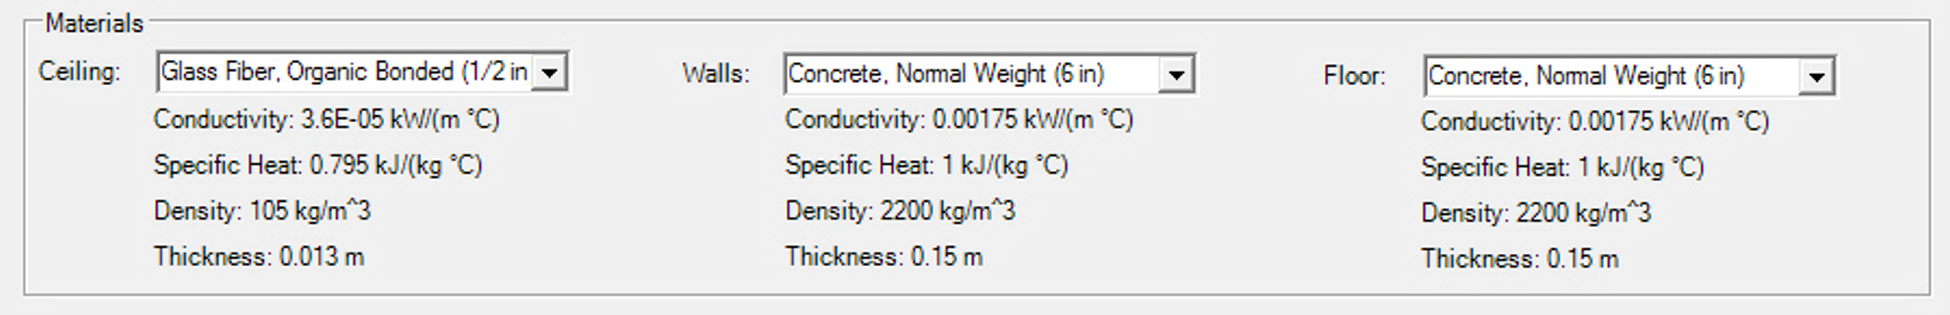
\includegraphics[width=6.5in]{FIGURES/Input_File/Compartment_Materials}
\end{figure}

The bounding surfaces are the ceilings, walls and floors that define a compartment. These are referred to as thermophysical boundaries, since each participates in conduction and radiation as well as defining the compartments, unless these phenomena are explicitly turned off. 

\textbf{Ceiling Material} (default value: Gypsum Board): material name from the thermal properties data file used for the ceiling surface of the compartment. 

\textbf{Wall Material} (default value: Gypsum Board): material name from the thermal properties data file used for the wall surfaces of the compartment.

\textbf{Floor Material} (default value: Off): material name from the thermal properties data file used for the floor surface of the compartment.

\begin{itemize}
\item If the thermophysical properties of the enclosing surfaces are not included, CFAST will treat them as adiabatic (no heat transfer).

\item If a name is used which is not in the database, the model should stop with an error message. The keyword in the data file simply gives a name (such as CONCRETE) which refers to the properties for that material in the thermal data file (see section 4.2.3 and Appendix A for details on the thermophysical database).

\item Since most of the heat conduction is through the ceiling, and since the conduction calculation takes a significant fraction of the computation time, it is recommended that initial calculations be made using the ceiling only.  Adding the walls generally has a small effect on the results, and the floor contribution is usually negligible.  Clearly, there are cases where the above generalization does not hold, but it may prove to be a useful screening technique. A caveat in including floor properties is that the set of equations describing heat transfer becomes difficult to solve once the thermal wave from the compartments reaches the unexposed side of a floor. The back surfaces of compartments are assumed to be exposed to ambient conditions unless specifically specified (see the section on Surface Connections) to specify heat transfer connections between compartments).
\end{itemize}

\section{Compartment Connections}

Flow through vents can be natural flow through doors, windows, or openings in ceilings and floors; or forced flow in a mechanical ventilation system.  Natural flow comes in two varieties.  The first is referred to as horizontal flow.  It is the flow which is normally thought of in discussing fires.  It encompasses flow through doors, windows and so on.  The other is vertical flow and can occur if there is a hole in the ceiling or floor of a compartment.  This latter phenomena is useful in some scenarios such as in a ship where openings in floors and ceilings through scuttles are common and in buildings with manual or automatic heat and smoke venting.

Flow through normal vents is governed by the pressure difference across a vent.  There are two situations which give rise to flow through vents.  The first is flow of air or smoke driven from a compartment by buoyancy.  The second type of flow is due to expansion which is particularly important when conditions in the fire environment are changing rapidly.  Rather than depending entirely on density differences between the two gases, the flow is forced by volumetric expansion.

In addition to natural flow, forced flow from mechanical ventilation can affect a fire as well. More important than affecting the fire, however, is the dispersal of the smoke and toxic gases from the fire to adjacent spaces, if ventilation continues to operate after a fire starts.

Atmospheric pressure is about 100 000 Pa. Fires produce pressure changes from 1 Pa to 1000 Pa and mechanical ventilation systems typically involve pressure differentials of about 1 Pa to 100 Pa.  In order to address pressure-induced flow, pressure differences of about 0.1 Pa out of 100 000 Pa for the overall problem or $10^{-4}$ Pa for adjacent compartments must be tracked.

The keywords which describe the various flow regimes are:

\begin{itemize}
\item Windows and doors (horizontal flow through vertical vents): HVENT, specifies vent which connect compartments horizontally
\item Holes in a ceiling/floor (vertical flow through horizontal vents: VVENT, specifies a vent which connects compartments vertically
\item HVAC specification: MVENT specifies a vent which connects compartments with a forced flow
\end{itemize}

For all three types of vents the size of the vent opening (expressed as a fraction of the original opening) may be changed:

\begin{itemize}
\item EVENT change the opening fraction of the specified vent at a chosen time.
\item RAMP change the opening fraction as a function of time by specifying a series of time and fraction pairs
\end{itemize}

Each of these commands is discussed in the sections that follow.

\subsection{Defining Natural Flow Connections Through Doors and Windows}

Horizontal flow connections may include doors between compartments or to the outdoors as well as windows in the compartments.  These specifications do not necessarily correspond to physically connecting the walls between specified compartments.  Rather, lack of an opening simply prevents flow between the compartments.  Horizontal flow connections may also be used to account for leakage between compartments or to the outdoors. 

Horizontal connections can only be created between compartments that physically overlap in elevation at some point. These may include doors between compartments or windows in the compartments (between compartments or to the outdoors).  Openings to the outside are included as openings to a compartment with a number one greater than the number of compartments described in the geometry section.  The relevant CFAST keyword is HVENT.  Details of the CFAST keywords are included in the appendix. It is possible to define a total of 25 horizontal flow connections between any pair of compartments. A number from 1 to 25 uniquely identifies the connection. This number is automatically assigned by the input editor based on the order they appear in the summary table on the horizontal flow vents page.

\begin{figure}[h!]
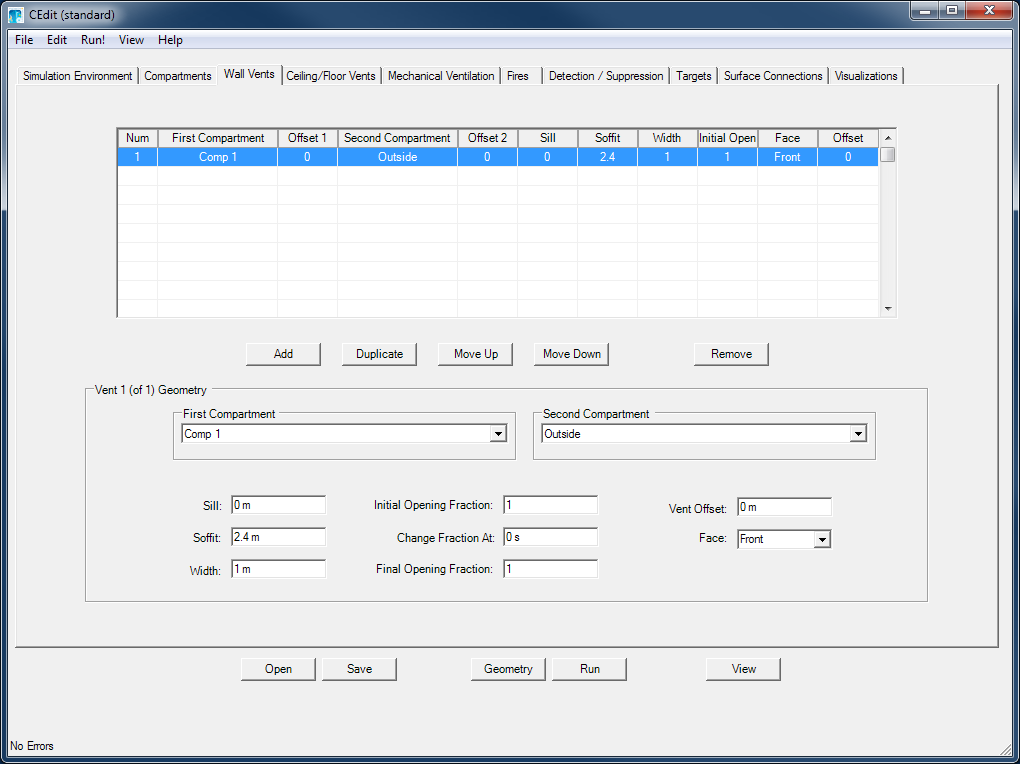
\includegraphics[width=6.5in]{FIGURES/Input_File/Natural_Flow_Tab}
\end{figure}

Most of the tabbed pages in the program are of similar design, with a summary of the defined items in table form at the top of the page, a series of buttons to add, remove, or modify the item highlighted in the summary table, and a number of individual inputs below which details all of the inputs for the item selected in the summary table. The buttons included on the horizontal flow vents page are as follows.

\begin{wrapfigure}{l}{0pt}
  
\includegraphics[width=0.781in]{FIGURES/Input_File/Add_Button}
\end{wrapfigure}

Use the Add button to create a new horizontal flow vent with default values for all entries. \\~ \\

\begin{wrapfigure}{l}{0pt}
  
\includegraphics[width=0.781in]{FIGURES/Input_File/Duplicate_Button}
\end{wrapfigure}

Use the Duplicate button to create a copy of the horizontal flow vent currently selected in the summary table at the top of the page. The new vent is added to the end of the list with the named changed to indicate it is a copy of the selected item. \\

\begin{wrapfigure}{l}{0pt}
  
\includegraphics[width=0.781in]{FIGURES/Input_File/Move_Up_Button}
\end{wrapfigure}

Use the Move Up and Move Down buttons to change the order of the list of horizontal flow vents in the summary table. This simply changes the automatically assigned vent numbers for the vents. Vents can be ordered as desired. \\~ \\

\begin{wrapfigure}{l}{0pt}
  
\includegraphics[width=0.781in]{FIGURES/Input_File/Remove_Button}
\end{wrapfigure}

Use the Remove button to delete the selected horizontal flow vent from the list of horizontal flow vents in the summary table.  Other vents are renumbered once the vent is deleted. \\~ \\

\begin{lstlisting}
HVENT,1,2,1,1,2.4,0,1,0,0,1,1
EVENT,H,1,2,1,120,1,1
\end{lstlisting}

\begin{figure}[h!]
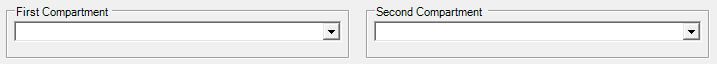
\includegraphics[width=6.5in]{FIGURES/Input_File/Compartment_From_To}
\end{figure}

\textbf{First Compartment:} First of the two compartments to be connected by a horizontal flow vent.  Compartments are numbered automatically by the input editor and by the model in the order they are read from the input data file and/or the order they appear in the summary table on the compartment geometry page. Compartment numbers begin with 1, so the first compartment is number 1, the second 2, and so forth.

\textbf{Second Compartment:} Second of the two compartments to be connected by a horizontal flow vent.  Compartments are numbered automatically by the input editor and by the model in the order they are read from the input data file and/or the order they appear in the summary table on the compartment geometry page. Compartment numbers begin with 1, so the first compartment is number 1, the second 2, and so forth.

There are also two parameters which are used to locate the compartments relative to each other. These are used to incorporate additional three dimensional information of the relative location of the vents with respect to each other. In the compartment view of CFAST, the orientation is that the rotation/translation point of the compartment is the back/bottom/left. In this view, both parameters would be with respect to the left hand side of the respective compartments. This allows the corridor filling model to incorporate a delay time for filling based on the separation between the vents. These parameters are needed only if the HALL command is used. 

\textbf{First Compartment Offset} (default units: m, Default value: 0 m): Horizontal distance between the centerline of this vent and the reference point in the first compartment.

\textbf{Second Compartment Offset } (default units: m, Default value: 0 m): Horizontal distance between the centerline of this vent and the reference point in the second compartment.

\begin{figure}[h!]
\begin{center}
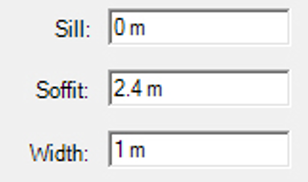
\includegraphics[width=1.1in]{FIGURES/Input_File/Vent_Size}
\end{center}
\end{figure}

\textbf{Sill} (default units: m, default value: none): Sill height is the height of the bottom of the opening relative to the floor of the compartment selected as the first compartment. 

\textbf{Soffit} (default units: m, default value: none): Position of the top of the opening relative to the floor of the compartment selected as the first compartment.   

\textbf{Width} (default units: m, default value: none): The width of the opening.

\begin{figure}[h!]
\begin{center}
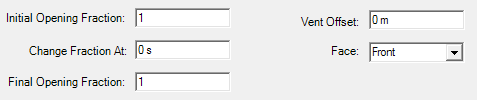
\includegraphics[width=3.1in]{FIGURES/Input_File/Vent_Open_Close}
\end{center}
\end{figure}

Horizontal flow vents may be opened or closed during the fire. The relevant CFAST keyword is EVENT. The initial format of EVENT is similar to HVENT specifying the connecting compartments and vent number.  Each EVENT line in the input file details the open/close time dependent characteristics for one horizontal flow vent by specifying a fractional value and a time.  The default is 1.0 which is a fully open vent.  A value of 0.5 would specify a vent which is halfway open.

\textbf{Initial Opening Fraction} (default value: 1): Flow through horizontal vents is calculated based on the area of the vent.  Normally, the vent is fully open.  If desired, the user may specify a fraction between 0 and 1 that allows the vent to be partially or fully closed at the beginning of the simulation.  In the model calculation, the vent width is multiplied by this fraction.  The opening fraction may be changed at any time in the simulation through the use of the EVENT command.

\textbf{Change Opening Fraction At Time}  (default units: s, default value: 0 s)  Time during the simulation at which to change the opening fraction.

\textbf{Final Opening Fraction} (default value: 1): for horizontal flow vents, the fraction specifies the fractional width opening of the vent. Fractional values must be between 0 and 1.

\textbf{Wind} (default value 0): The wind coefficient is the cosine of the angle between the wind vector and the vent opening.  This applies only to vents which connect to the outside.  The range of values is -1.0 to 1.0.  In the input editor, this is specified as the angle between the face of the vent and the wind direction.

\textbf{Face:} For visualization, FACE specifies which wall the vent will be displayed on in smokeview.  Choices are Front, Rear, Right, Left and are relative to the X-Z plane.

\begin{itemize}
\item The soffit and sill specifications are with respect to the first compartment specified and is not necessarily symmetric since the elevation of the second compartment may be different than the first.  Reversing the order of the compartment designations does make a difference.
\end{itemize}

\subsection{Defining Natural Flow Connection Through Ceiling and Floor Openings}

This section of the input data file describes these vertical flow openings. Examples of these openings are scuddles in a ship, or a hole in the roof of a residence. Combined buoyancy- and pressure-driven (i.e., forced) flow through a vertical flow vent is possible when the connected spaces adjacent to the vent are filled with gases of different density in an unstable configuration, with the density of the top space larger than that of the bottom space. With a moderate cross-vent pressure difference, the instability leads to a bi-directional flow between the two spaces. For relatively large cross-vent pressure difference the flow through the vent is unidirectional, from the high- to the low-pressure space. 
Connections can exist between compartments or between a compartment and the outdoors. Openings to the outside are included as openings to a compartment with a number one greater than the number of compartments defined in the scenario.  These connections are described by the VVENT keyword. Each VVENT line in the input file describes one vertical vent.  There are four parameters which include each of the connected compartments, the shape of the opening, and the effective area of the vent.

\begin{figure}[h!]
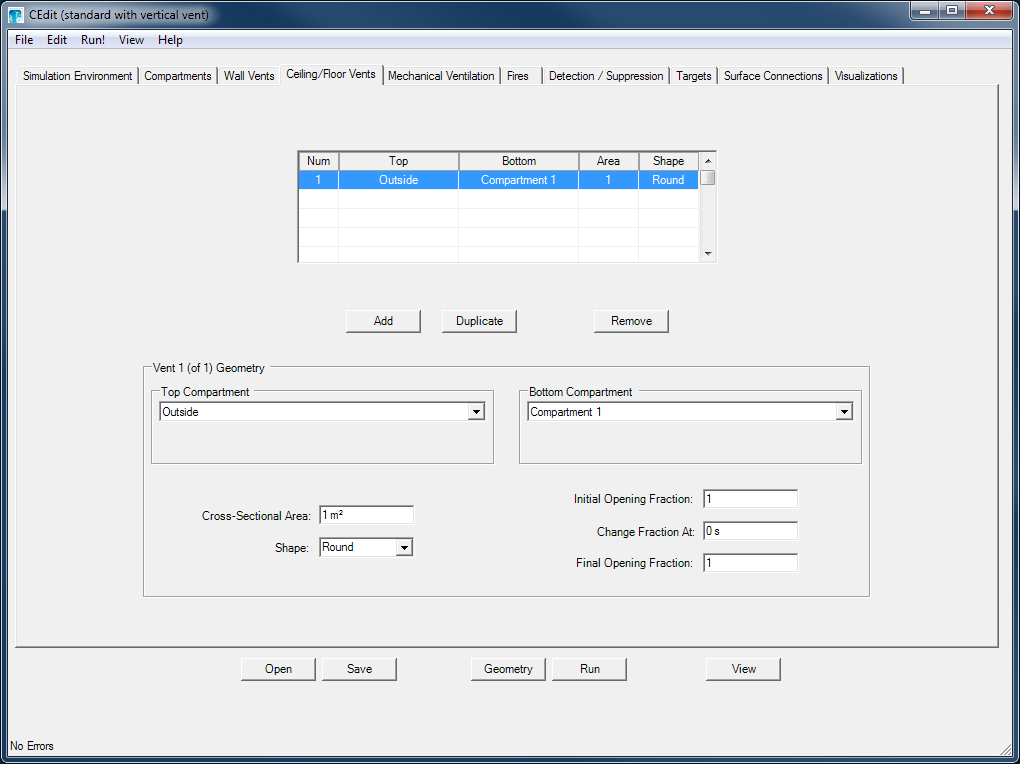
\includegraphics[width=6.5in]{FIGURES/Input_File/Vertical_Flow_Tab}
\end{figure}
 
Most of the tabbed pages in the program are of similar design, with a summary of the defined items in table form at the top of the page, a series of buttons to add, remove, or modify the item highlighted in the summary table, and a number of individual inputs below which details all of the inputs for the item selected in the summary table. The buttons included on the vertical flow vents page are as follows.

\begin{wrapfigure}{l}{0pt}
  
\includegraphics[width=0.781in]{FIGURES/Input_File/Add_Button}
\end{wrapfigure}

Use the Add button to create a new vertical flow vent with default values for all entries. \\~ \\

\begin{wrapfigure}{l}{0pt}
  
\includegraphics[width=0.781in]{FIGURES/Input_File/Duplicate_Button}
\end{wrapfigure}

Use the Duplicate button to create a copy of the vertical flow vent currently selected in the summary table at the top of the page. The new vent is added to the end of the list with the named changed to indicate it is a copy of the selected item. \\

\begin{wrapfigure}{l}{0pt}
  
\includegraphics[width=0.781in]{FIGURES/Input_File/Remove_Button}
\end{wrapfigure}

Use the Remove button to delete the selected vertical flow vent from the list of vertical flow vents in the summary table.  Other vents are renumbered once the vent is deleted. \\~ \\

\begin{lstlisting}
VVENT,2,1,2.44,2,1
EVENT,V,1,2,1,120,1,1
\end{lstlisting}

\textbf{Top Compartment:} The top or first of the two compartments to be connected by a vertical flow vent. The vent is through the floor of this compartment.  Compartments are numbered automatically by the input editor and by the model in the order that they are read from the input data file and/or the order they appear in the summary table on the compartment geometry page. Compartment numbers begin with 1, so the first compartment is number 1, the second 2, and so forth.

\textbf{Bottom Compartment:} The bottom or second of the two compartments to be connected by a horizontal flow vent. The vent is through the ceiling of this compartment. Compartments are numbered automatically by the input editor and by the model in the order they are read from the input data file and/or the order they appear in the summary table on the compartment geometry page. Compartment numbers begin with 1, so the first compartment is number 1, the second 2, and so forth.

\textbf{Cross-sectional Area} (default units: m$^2$, default value: none): specifies the cross-sectional area of the vent connecting the two compartments.

\textbf{Shape:} The shape factor is 1 for circular openings and 2 for square openings.

\textbf{Initial Opening Fraction:} Flow through vertical vents is calculated based on the area of the vent.  Normally, the vent is fully open.  If desired, the user may specify a fraction between 0 and 1 that allows the vent to be partially or fully closed at the beginning of the simulation.  In the model calculation, the vent area is multiplied by this fraction.  The opening fraction may be changed at any time in the simulation through the use of the EVENT command.

\textbf{Change Opening Fraction At Time} (default units: s, default value: 0 s): Time during the simulation at which to change the opening fraction.

\textbf{Final Opening Fraction:} for vertical flow vents, the fraction specifies the fractional cross-sectional area of the vent. Fractional values must be between 0 and 1.

\begin{itemize}
\item Although obvious, note that the top or first compartment must be the compartment on top of the bottom or second compartment.
\item CFAST allows only a single connection between any pair of compartments included in a simulation. This limitation is based on the implementation of the vertical flow algorithm in CFAST and on the validation efforts for the original algorithm development  which only studied a single opening between connected compartments.
\item Vertical connections can only be created between compartments that could be physically stacked based on specified floor and ceiling elevations for the compartments.  Some overlap between the absolute floor height of one compartment and the absolute ceiling height of another compartment is allowed.  However, whether the compartments are stacked or overlap somewhat, the ceiling/floor absolute elevations must be within 0.01 m of each other. The check is not done when the connection is to the outside.
\end{itemize}

\subsection{Defining Mechanical Ventilation Connections}

Fan-duct systems are commonly used in buildings for heating, ventilation, air conditioning, pressurization, and exhaust. Generally, systems that maintain comfortable conditions have either one or two fans.  Residences often have a systems with a single fan. Further information about these systems is presented in  Klote and Milke \cite{Klote:2002} and the American Society of Heating, Refrigerating and Air Conditioning Engineers \cite{ASHRAE:2001}.

\begin{figure}[h!]
\begin{center}
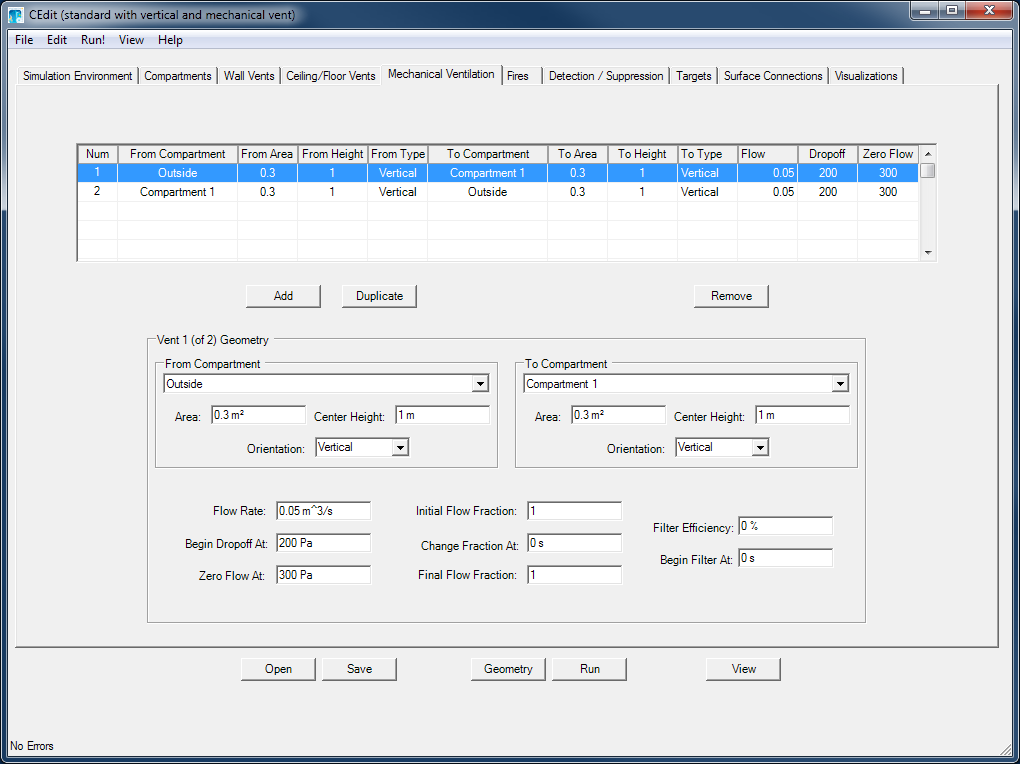
\includegraphics[width=6.5in]{FIGURES/Input_File/Mechanical_Vent_Tab}
\end{center}
\end{figure}

The model for mechanical ventilation used in CFAST is based on the theory of networks and is based on the model developed by Klote \cite{Klote:1988a}.  This is a simplified form of Kirchoff's law which says that flow into a node must be balanced by flow out of the node. The equations used describe the relationship between the pressure drop across a duct, the resistance of a duct, and the mass flow.  The pressure can be changed by conditions in a compartment, or a fan in line in the duct system.  Resistance arises from the finite size of ducts, roughness on duct surfaces, bends and joints. In CFAST, default values are used for the duct properties, and thus mechanical ventilation connections are simply described by the connections to the two compartments and a fan whose throughput is a constant volumetric flow up to a user-specified pressure drop across the fan, dropping to zero at high backwards pressure on the fan.

Most of the tabbed pages in the program are of similar design, with a summary of the defined items in table form at the top of the page, a series of buttons to add, remove, or modify the item highlighted in the summary table, and a number of individual inputs below which details all of the inputs for the item selected in the summary table. The buttons included on the mechanical flow vents page are as follows.

\begin{wrapfigure}{l}{0pt}
  
\includegraphics[width=0.781in]{FIGURES/Input_File/Add_Button}
\end{wrapfigure}

Use the Add button to create a new mechanical flow vent with default values for all entries. \\~ \\

\begin{wrapfigure}{l}{0pt}
  
\includegraphics[width=0.781in]{FIGURES/Input_File/Duplicate_Button}
\end{wrapfigure}

Use the Duplicate button to create a copy of the mechanical flow vent currently selected in the summary table at the top of the page. The new vent is added to the end of the list with the named changed to indicate it is a copy of the selected item. \\

\begin{wrapfigure}{l}{0pt}
  
\includegraphics[width=0.781in]{FIGURES/Input_File/Remove_Button}
\end{wrapfigure}

Use the Remove button to delete the selected mechanical flow vent from the list of vertical flow vents in the summary table.  Other vents are renumbered once the vent is deleted. \\~ \\

\begin{lstlisting}
MVENT,2,3,1,V,0.6,0.4225,V,0.75,0.0731,0.167,2000,3000,1
\end{lstlisting}

\begin{figure}[h!]
\begin{center}
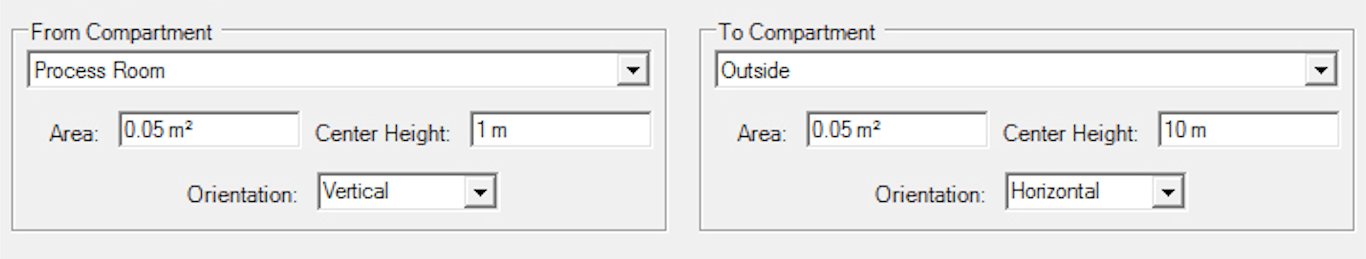
\includegraphics[width=4.553in]{FIGURES/Input_File/Mechanical_Vent_From_To}
\end{center}
\end{figure}
 
\textbf{From Compartment:} The first compartment to which the mechanical ventilation system diffuser is connected. Fan flow is from this compartment.  Compartments are numbered automatically by the input editor and by the model in the order they are read from the input data file and/or the order they appear in the summary table on the compartment geometry page. Compartment numbers begin with 1, so the first compartment is number 1, the second 2, and so forth.

\textbf{From Compartment Area} (default units: m$^2$, default value: none): Cross-sectional area of the opening into the compartment. The area will be truncated if the midpoint (height) is set such that the height plus or minus the effective length is above the compartment ceiling or below the floor.

\textbf{From Compartment Height} (default units: m, default value: none): Height of the duct opening above the floor of the compartment measured from the midpoint of the register.

\textbf{From Compartment Orientation:} The orientation of the diffuser relative to the floor of the compartment.  A horizontal diffuser implies vertical flow through the ceiling or floor of the compartment.  A vertical diffuser implies horizontal flow through a wall of the compartment.

\textbf{To Compartment:} The bottom or second of the two compartments to be connected by a horizontal flow vent. The vent is through the ceiling of this compartment. Compartments are numbered automatically by the input editor and by the model in the order they are read from the input data file and/or the order they appear in the summary table on the compartment geometry page. Compartment numbers begin with 1, so the first compartment is number 1, the second 2, and so forth.

\textbf{To Compartment Area} (default units: m$^2$, default value: none): Cross-sectional area of the opening into the compartment. The area will be truncated if the midpoint (height) is set such that the height plus or minus the effective length is above the compartment ceiling or below the floor.

\textbf{To Compartment Height} (default units: m, default value: none): Height of the duct opening above the floor of the compartment measured from the midpoint of the register.

\textbf{To Compartment Orientation:} The orientation of the diffuser relative to the floor of the compartment.  A horizontal diffuser implies vertical flow through the ceiling or floor of the compartment.  A vertical diffuser implies horizontal flow through a wall of the compartment.

\begin{figure}[h!]
\begin{center}
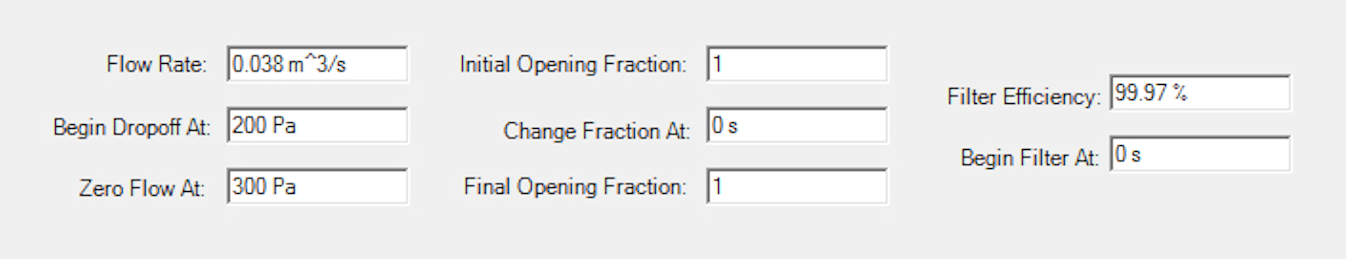
\includegraphics[width=4.487in]{FIGURES/Input_File/Mechanical_Vent_Flowrate}
\end{center}
\end{figure}

\textbf{Flow Rate} (default units: m$^3$/s, default value: none): Constant flow rate of the forced-air flow from the first compartment to the second compartment.

\textbf{Begin Drop Off Pressure} (default units: Pa, default value: 200 Pa): The description of the fan includes a drop off in flow beginning at a pressure specified by the user.  Above this pressure drop, the flow gradually drops to zero flow.

\textbf{Zero Flow Pressure} (default units: Pa, default value: 300 Pa): Specifies the pressure above which the flow through the mechanical ventilation connection is zero.

\textbf{Initial Opening Fraction:} Flow through mechanical vents is calculated based on the area of the vent.  Normally, the vent is fully open.  If desired, the user may specify a fraction between 0 and 1 that allows the vent to be partially or fully closed at the beginning of the simulation.  In the model calculation, the fan flow rate is multiplied by this fraction.  The opening fraction may be changed at any time in the simulation through the use of the EVENT command.

\textbf{Change Opening Fraction At Time} (default units: s, default value: none): Time during the simulation at which to change the opening fraction.

\textbf{Final Opening Fraction:} for mechanical flow vents, the fraction specifies the fractional fan flow rate for the vent. Fractional values must be between 0 and 1.

\textbf{Filter Efficiency} (default units:~\%, default value: none): Flow through mechanical vents may include filtering that removes a user-specified portion of soot and trace species mass from the flow through the vent.  By default, there is no filtering applied, that is all of the soot and trace species mass in the vent flow is passed through the vent. Within the user interface, this is specified as a filter efficiency of 0~\%.  If desired, the user may specify the fraction of the soot and trace species mass to be removed as a percentage.

\textbf{Begin Filtering At Time} (default units: s, default value: none): Time during the simulation at which the mechanical vent filtering begins.

\begin{itemize}
\item CFAST does not include provisions for reverse flow through a fan. Calibration for backward flow is not provided by fan manufacturers, so the equations incorporated in CFAST do not allow for such flow. The problem is simply that in this flow regime, the fan has stalled, and likely will soon fail. 
\item If the simulation includes mechanical ventilation filtering, care should be taken in choosing trace species production rates to insure the production rate is small compared to the total pyrolysis rate.  This will allow appropriate conservation of mass in the solution of the system of differential equation.  For large production rates of trace species, scaling factors can be used (e.g., divide by 1000) for the trace species production rate to reduce the relative magnitude compared to the pyrolysis rate.  For analysis, the resulting trace species in compartments and filters can be converted back to original units multiplying by the scaling factor used.
\end{itemize}

\section{Prescribing Fires}

A simulated fire in CFAST is implemented as a source of fuel mass which is released at a prescribed rate (the pyrolysis rate). Energy is released by the fuel and combustion products are created as it burns. In the fire, species production is calculated based on production yields prescribed by the user. In addition, the pyrolysis rate and resulting energy and species generation may be limited by the oxygen available for combustion. When sufficient oxygen is available for combustion, the heat release rate for the constrained fire is the same as for the unconstrained fire.

The model can simulate multiple fires in one or more compartments of the building.  These fires are treated as totally separate entities, with no interaction of the plumes. These fires are generally referred to as “objects” and can be ignited at a prescribed time, temperature or heat flux.

CFAST does not include a pyrolysis model to pre¬dict fire growth. Rather, pyrolysis rates for each fire are prescribed by the user.  ¬While this approach does not directly account for increased pyrolysis due to radiative feedback from the flame or com¬part¬ment, in theory these effects could be prescribed by the user as described in this section.  In an actual fire, this is an important consideration, and the specification used should consider the experimental conditions as closely as possible.

A fire releases energy based on the pyrolysis of fuel, but may be constrained by the oxygen available for combustion depending on the compartment conditions. Complete burning will take place only where there is suffi¬cient oxygen.  When insufficient oxygen is entrained into the fire plume, unburned fuel will be transported from zone to zone until there is sufficient oxygen and a high enough temperature to support combustion.  In general, CFAST uses a simple definition of a combustion reaction that includes major products of combustion for hydrocarbon fuels:
\be  \mathrm{C_{n_\C}H_{n_H}O_{n_O}N_{n_N}Cl_{n_{Cl}}} +  \nu_\OTWO \, \mathrm{O_2}  \rightarrow  \nu_\COTWO \, \mathrm{CO_2} + \nu_\HTWOO \, \mathrm{H_2O} + \nu_\CO \, \mathrm{CO} +
     \nu_\So \, \mathrm{Soot}  + \nu_\HCl \mathrm{HCl} + \nu_\HCN \mathrm{HCN} \label{stoich} \ee
assuming that all the nitrogen and chlorine in the fuel are converted to HCN and HCl. The stoichiometric coefficients $\nu_\So$, $\nu_\CO$, etc. represent appropriate molar ratios for a stoichiometric balance of the equation. For complete combustion of the simplest hydrocarbon fuel, methane reacts with oxygen to form carbon dioxide and water. The only inputs required are the fuel composition, heat release rate, and heat of combustion. For fuels that contain oxygen, nitrogen, or chlorine, the reaction becomes more complex. Stoichiometry is used to insure conservation of mass and elements in the reaction. The species which are calculated are oxygen, carbon dioxide, carbon monoxide, water, total unburned hydrocarbons (tuhc), and soot. Gaseous nitrogen is included, but only acts as a diluent. 

Production of hydrogen cyanide and hydrogen chloride are tracked solely based on user prescribed yields.  

The heat release rate for a constrained fire may be reduced below its prescribed value based upon the oxygen available for combustion. For the constrained fire, the burning rate may be less than the pyrolysis rate and cannot be simplified as in the case of the unconstrained fire. As fuel and oxygen are consumed, heat is released and various products of combustion are formed.

For a constrained fire, the heat release rate is limited by available oxygen. This limit is applied in three places: The first is burning in the portion of the plume which is in the lower layer of the room of fire origin; the second is the portion of the plume in the upper layer, also in the room of origin; the third is in the vent flow which entrains air from a lower layer into an upper layer in an adjacent compartment. The unburned hydrocarbons are tracked in this model. Combustion of CO to CO$_2$ is not included in the model. Actual combustion chemistry is not considered in CFAST due to the complexities associated with detailed kinetics and transport.

There are two calculations involving radiation in this model. One is for energy balance and is based on broadband radiation absorption. The amount of radiation absorbed in sensitive to the species present, specifically water vapor, soot and carbon dioxide. The other is for visibility of egress signs. This calculation is based solely on the soot volume fraction and is reported as optical depth (per meter). The conversion factor is based on the recent work by Mulholland and Croarkin \cite{Mullholland:2000}. The value for converting mass density in kg/m3 to optical depth is 3817 m$^2$/kg. The value reported is intended specifically for assessing the visibility of egress signs, based on the work of Jin \cite{Jin:1979}.  It is not applicable to the far blue or red regions of the spectrum and so should not be used for assessing optical detection of fires through smoke.

\newpage

\begin{figure}[h!]
\begin{center}
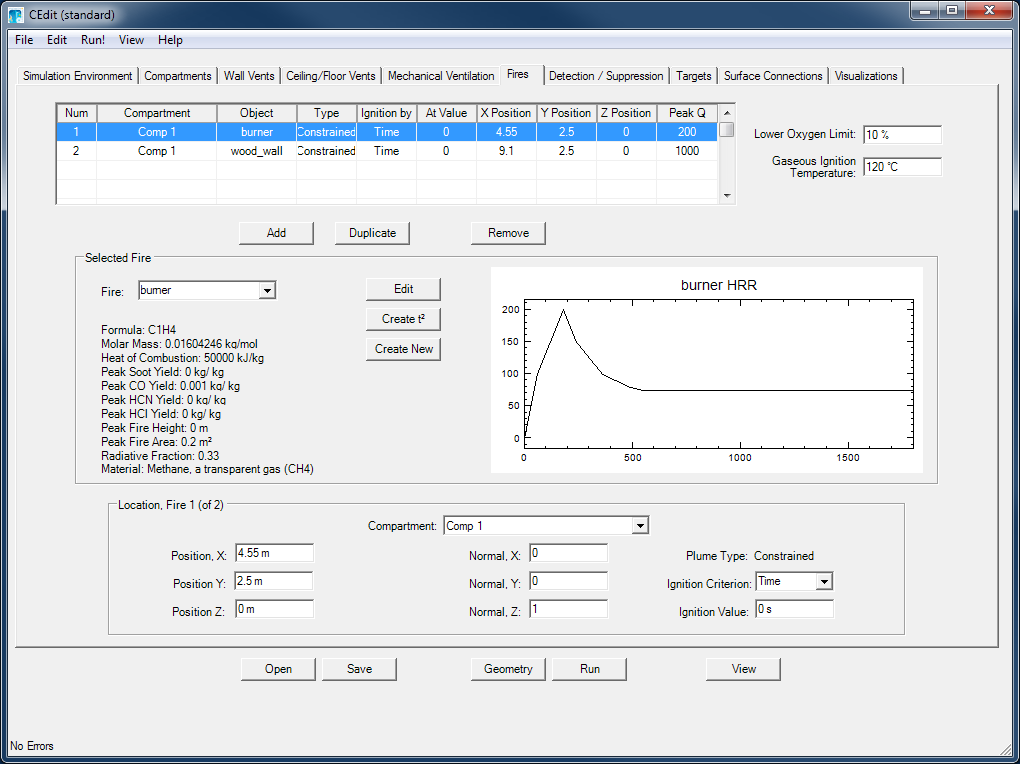
\includegraphics[width=6.5in]{FIGURES/Input_File/Fire_Tab}
\end{center}
\end{figure}
 
Most of the tabbed pages in the program are of similar design, with a summary of the defined items in table form at the top of the page, a series of buttons to add, remove, or modify the item highlighted in the summary table, and a number of individual inputs below which details all of the inputs for the item selected in the summary table. The buttons included on the fires page are as follows.


\begin{wrapfigure}{l}{0pt}
  
\includegraphics[width=0.781in]{FIGURES/Input_File/Add_Button}
\end{wrapfigure}

Use the Add button to create a new fire with default values for all entries. \\~ \\

\begin{wrapfigure}{l}{0pt}
  
\includegraphics[width=0.781in]{FIGURES/Input_File/Duplicate_Button}
\end{wrapfigure}

Use the Duplicate button to create a copy of the fire currently selected in the summary table at the top of the page. The new fire is added to the end of the list with the named changed to indicate it is a copy of the selected item. \\

\begin{wrapfigure}{l}{0pt}
  
\includegraphics[width=0.781in]{FIGURES/Input_File/Remove_Button}
\end{wrapfigure}

Use the Remove button to delete the selected fire from the list of vertical flow vents in the summary table.  Other fires are renumbered once the fire is deleted. \\~ \\

\begin{lstlisting}
!!Wood_Wall
FIRE,1,4.55,2.5,0,1,1,0,0,0,1,Wood_Wall
CHEMI,1,4,0,0,0,0.33,1.81E+07,HARDWOOD
TIME,0,8000
HRR,0,1000000
SOOT,0.02,0.02
CO,0.02,0.02
TRACE,0,0
AREA,0.05,9
HEIGH,0,3
\end{lstlisting}

\subsection{Global Fire Inputs}

Three inputs on the Fire Tab are global, that is, they apply to all fires included in a simulation.

\begin{wrapfigure}{l}{0pt}
  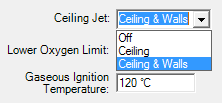
\includegraphics[width=0.781in]{FIGURES/Input_File/Ceiling_Jet}
\end{wrapfigure}

\textbf{Ceiling Jet}: If the fire is large enough, the plume from the fire will penetrate the upper layer, impinge on the ceiling surface, and increase the convective heat transfer to the ceiling or increase the temperature nearby targets or detectors near the ceiling.  CFAST includes an algorithm to account for some of these effects.  Details of the inputs are included in the section on ceiling jets included in the Special Features chapter, below.

\begin{wrapfigure}{l}{0pt}
  
\includegraphics[width=0.781in]{FIGURES/Input_File/LOL}
\end{wrapfigure}

\textbf{Lower Oxygen Limit} (default units: \%, default value: 10~\%):  In the CFAST model, a limit is incorporated by limiting the burning rate as the oxygen level decreases until a ``lower oxygen limit'' (LOL) is reached. The lower oxygen limit is incorporated through a smooth decrease in the burning rate near the limit. Normally, this value would not be changed by the user.

\begin{wrapfigure}{l}{0pt}
  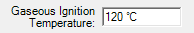
\includegraphics[width=0.781in]{FIGURES/Input_File/Gaseous_Ignition_Temperature}
\end{wrapfigure}

\textbf{Gaseous Ignition Temperature} (default units: \degc, default value: ambient temperature plus 100 K): The lower temperature limit on the burning of fuel in a gas layer. Since CFAST does not support a combustion kinetics model, this is the algorithm used for fires out of vents.  Normally, this value would not be changed by the user.

\subsection{Defining Individual Fires}

Fires in CFAST are defined as a series of individual fire objects which are then placed as desired in compartments in a simulation.

Each fire object defines the time dependent variables of the fire are described by the mass loss rate, rate of heat release, fuel height, and fuel area inputs.  Species production rates are specified in a manner similar to the fire, entering the rates as a series of points with respect to time.  The species which are followed by CFAST are: carbon dioxide, carbon monoxide, hydrogen cyanide, hydrogen chloride, nitrogen, oxygen, soot, total unburned hydrocarbons and water. There is a separate calculation of the concentration-time product Ct. Finally, a user-specified trace species can be specified to follow the transport that results from fire-induced flow for an arbitrary species. This may be of particular interest for radiological releases \cite{Jones:2008}, but may be useful for any trace amounts released by a fire.

Each fire object is defined in a separate comma-separated spreadsheet file with an extension of ``.o' and saved in the CFAST input file for the current simulation. As many fire objects as desired may be defined by the user.  At least one fire in the simulation should ignite at a user-specified time.  Other fire objects can ignite based on time, temperature or heat flux conditions.

\begin{figure}[h!]
\begin{center}
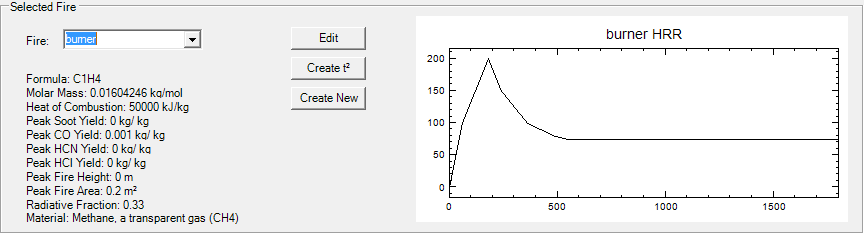
\includegraphics[width=6.5in]{FIGURES/Input_File/Fire_Object_Plot}
\end{center}
\end{figure}

\begin{wrapfigure}{l}{0pt}
  
\includegraphics[width=0.781in]{FIGURES/Input_File/Edit_Button}
\end{wrapfigure}

Use the Edit button to edit the currently selected fire object. Fire Objects can also be changed from the Tools menu. A separate window allows the user to view or change any of the available fire objects. Details of fire inputs for a fire is included below. \\~ \\

\begin{wrapfigure}{l}{0pt}
  
\includegraphics[width=0.781in]{FIGURES/Input_File/Create_t2_Button}
\end{wrapfigure}

Use the Add t$^2$ button to create a new fire object with a heat release rate specified by the user in the form of a t-squared fire.  For a wide range of fires, the fire growth can be accurately represented with a power law relation of the form $\dQ=\alpha t^2$  where $\dQ$  is the heat release rate of the fire, $\alpha$ is the fire intensity coefficient, and $t$ is time \cite{Schifiliti:2002}. A set of specific t-squared fires labeled slow, medium, and fast, with fire intensity coefficients ($\alpha$) such that the fires reached 1054 kW (1000 BTU/s) in 600 s, 300 s, and 150 s, respectively were proposed for design of fire detection systems .  Later, these specific growth curves and a fourth called "Ultra-fast" which reaches 1054 kW in 75 s, gained favor in general fire protection applications. A separate window allows the user to define the t-squared fire. Details of the inputs for a t-squared fire is included below.
 

\begin{wrapfigure}{l}{0pt}
  
\includegraphics[width=0.781in]{FIGURES/Input_File/Create_New_Button}
\end{wrapfigure}

Use the Create New button to create a new fire object with default values for all entries.  No time-dependent values are included in the new fire.  \\~ \\

\begin{figure}[h!]
\begin{center}
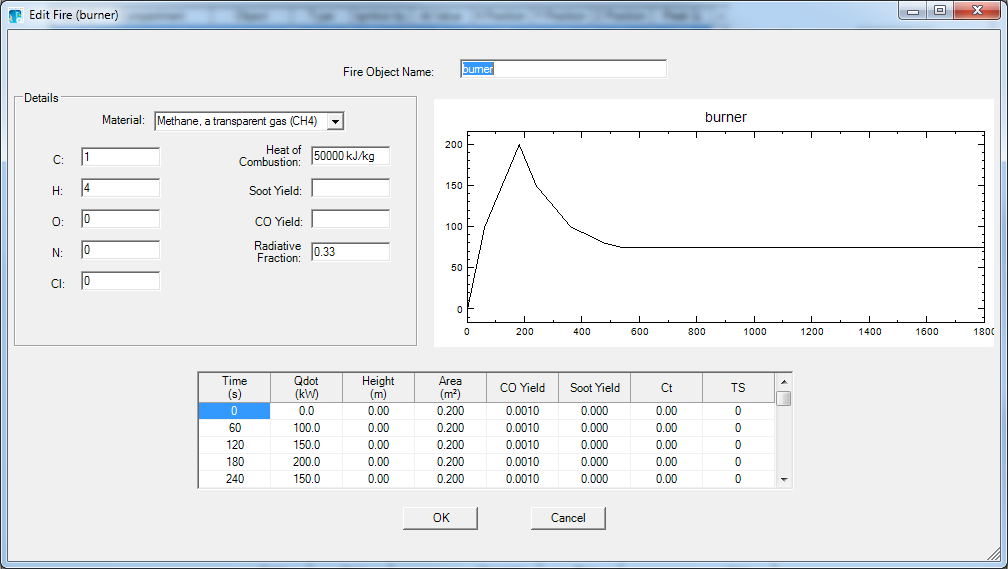
\includegraphics[width=6.5in]{FIGURES/Input_File/Fire_Object_Edit}
\end{center}
\end{figure}

\textbf{Fire Name:} The name from the collection of fire objects for the desired object.  This corresponds to the name of the fire object file, without the extension. Specifying a name not found in the database causes CFAST to stop with an appropriate error message.

\textbf{Material} (default value: none): material name from the thermal properties data file used for the object. The material properties are used to calculate heat transfer into the object from its surroundings.

\textbf{C, H, O, N, Cl}: Molecular formula of the burning fuel. Burning fuels in CFAST are assumed to be hydrocarbon fuels that contain at least Carbon and Hydrogen and optionally Oxygen, Nitrogen, and Chlorine. These five inputs define the stoiciometry of the fuel as it is burned.  Thus, for example, all of the specified Nitrogen and Chlorine is assumed to completely react to form HCN and HCl.  If only partial conversion is desired, a smaller ratio for Nitrogen and/or Chlorine can be specified.

\textbf{Heat of Combustion} (default units: J/kg, default value: 50 000 000 J/kg): The energy released per kilogram of mass burned.

\textbf{Soot Yield} (default units: kg/kg, default value: 0 kg/kg): Constant species yields of soot expressed as ratios of carbon to fuel produced by the pyrolysis of the fuel. This input allows the user to specify a single value for soot yield for all time points in the fire time line. Individual time points can be changed as desired in the spreadsheet input described below.

\textbf{CO Yield} (default units: kg/kg, default value: determined by

\textbf{Radiative Fraction}: The fraction of the energy produced in combustion that is radiated from the fire and plume. Within CFAST, the radiative fraction defaults to 0.30 ; i.e., 30 \% of the fire’s energy is released via radiation.  For other fuels, the work of Tewarson \cite{Tewarson:2003}, McCaffrey \cite{McCaffrey:1982}, or Koseki \cite{Koseki:1989} is available for reference.  The typical range for the radiative fraction is from about 0.05 to 0.4.

\chapter{Output from CFAST}
\label{Output_Chapter}

The output of CFAST includes the temperatures of the upper and lower gas layers within each compartment, the ceiling/wall/floor temperatures within each compartment, the visible smoke and gas species concentrations within each layer, target temperatures and sprinkler activation time.  The amount of information can be very large, especially for complex geometries and long simulations.

\section{Compact Output}

The default output to the console is called the compact form, and shows the basic information about a scenario, including layer temperatures and the size of fires. Default text output provides a simple overview for the user to make sure the case runs as expected.
\begin{lstlisting}[basicstyle=\scriptsize]
 Time =   1800.0 seconds.

 Compartment   Upper   Lower   Inter.  Pyrol     Fire      Pressure  Ambient
               Temp.   Temp.   Height  Rate      Size                Target
               (C)     (C)     (m)     (kg/s)    (W)       (Pa)      (W/m^2)
 -----------------------------------------------------------------------------
    1          113.4    33.3    1.4     1.393E-02 3.000E+05-0.790      523.
  Outside                                         0.00
\end{lstlisting}
The first column contains the compartment number.  On each row with its compartment number from left to right is the upper layer temperature, lower layer temperature, the height of the interface between the two layers, the total pyrolysis rate, and finally the total fire size.  The only value given for the outside is the total heat release rate of fires venting to the outside.

\section{Detailed Outputs}

The following sections describe each of the outputs from the model.  Each section refers to a specific part of the print out and appears in the order the output appears. A description of each option follows.

\subsection{Output for Initialization}

This option prints the initial conditions to the output before the actual run starts.  This merely mimics the inputs specified by the user in the input data file  The initial conditions brake down into seven sections.  Each is described below with the section name. The following explanation uses the output from the case STANDARD.IN. STANDARD.IN is included in the distribution. Please note, there are no mechanical ventilation, horizontal vents or detectors in this example, so the section discussing these phenomena are from additional data files.

\subsubsection{Overview}

The overview gives a general description of the case.  The output is fairly self explanatory. ``Doors, ...'' is the total number of horizontal natural flow vent connections in all compartments of the simulation.  ``Ceil. Vents, ...'' gives the total number of vertical natural flow vent connections in all compartments of the simulation.  The last header on the line ``MV Connections'' has the total number mechanical flow connections to all compartments in the simulation. Times in these outputs come from the TIMES input. All times are in s.
\begin{lstlisting}[basicstyle=\scriptsize]
 OVERVIEW


 Compartments    Doors, ...    Ceil. Vents, ...    MV Connects
    1               1             0                    0

 Simulation     Output         Smokeview      Spreadsheet
 Time           Interval       Interval       Interval
 (s)            (s)            (s)            (s)
   1800         120             10             30
\end{lstlisting}

\subsubsection{Ambient Conditions}

This section, like the overview section, needs little elaboration.  It gives the starting atmospheric conditions for the simulation both for outside and inside the structure. Data for these outputs come from the TAMB and EAMB inputs. Temperatures are in K, pressure in Pa, elevations in m, and wind speed in m/s. Wind Power is the dimensionless power law coefficient from the WIND input.
\begin{lstlisting}[basicstyle=\scriptsize]
 AMBIENT CONDITIONS

 Interior       Interior       Exterior       Exterior
 Temperature    Pressure       Temperature    Pressure
   (C)            (Pa)           (C)            (Pa)

     20.          101300.          20.          101300)
\end{lstlisting}

\subsubsection{Compartments}

The compartments section gives a summary of the geometry for the simulation.  A simple table summarizes the geometry with compartments running down the page in numerical order.  The various dimensions for each compartment are on the row with its compartment number.  Two columns need explanation.  The second to last column ``Ceiling Height'' gives the height of the ceiling relative to the station height in the Ambient Conditions section.  Similarly the ``Floor Height'' refers to the height of the floor above the station height.

\begin{lstlisting}[basicstyle=\scriptsize]
COMPARTMENTS

Compartment  Name                Width        Depth        Height       Ceiling      Floor
                                                                        Height       Height
                                 (m)          (m)          (m)          (m)          (m)
------------------------------------------------------------------------------------------------
    1        Compartment 1        9.10         5.00         4.60         4.60         0.00
\end{lstlisting}


\subsubsection{Horizontal Natural Ventilation}

This is the first table in the vent connections section.  Each row in the table characterizes one vent.  The first two columns contain the two compartments connected by the vent.  Each vent is ordered first by the lower number of the two compartments and then the numeric order of the second compartment.  The third column gives the vent number.  Column four is the width of the vent.  The next two columns report the sill and soffit height for the vent relative to the floor of the first compartment.  The seventh and eighth columns have a second listing of the sill and soffit height, this time relative to the station height.  Area of the vent is in the last column.

\begin{lstlisting}[basicstyle=\scriptsize]
VENT CONNECTIONS

Horizontal Natural Flow Connections (Doors, Windows, ...)

From           To             Vent       Width       Sill        Soffit      Abs.        Abs.
Compartment    Compartment    Number                 Height      Height      Sill        Soffit
                                         (m)         (m)         (m)         (m)         (m)
----------------------------------------------------------------------------------------------------
Compartment 1   Outside        1          1.00        0.00        2.40        0.00        2.40
\end{lstlisting}
From compartment, to compartment, vent number, width, sill height, and soffit height all come directly from the HVENT specifications in the input data file. Absolute sill height and absolute soffit height is the station elevation + compartment floor height + sill height. Absolute soffit height and absolute soffit height is the station elevation + compartment floor height + soffit height

\subsubsection{Vertical Natural Ventilation}

The first column is the upper compartment.  The upper compartment is the compartment where the vent opens into the floor.  The second column is the lower compartment where the vent is in the ceiling.  The third column describes the shape of the vent, which can be either round or square.  The fourth column gives the area of the vent.  The last two columns are the height of the vent, relative to the floor of the lower room and relative to the station height respectively.
\begin{lstlisting}[basicstyle=\scriptsize]
Vertical Natural Flow Connections (Ceiling, ...)

Top            Bottom         Shape     Area      Relative  Absolute
Compartment    Compartment                        Height    Height
                                        (m^2)     (m)       (m)
----------------------------------------------------------------------
 Outside           1          Round      1.00      4.60      4.60
\end{lstlisting}
Top compartment, bottom compartment, shape, and area come from the VVENT specifications in the input data file. Relative height is the height of the vent above the floor of the bottom compartment and absolute height is the height of the vent above the station elevation.

\subsubsection{Mechanical Flow Connections}

This section lists all connections to compartments and fans that connect between compartments. The first five columns in the fan table appear almost the same as the connections and ducts table.  The table lists, in order, the number of the system the fan is a part, the ``from'' node and its height, the ``to'' node and its height.  A fan actually draws air from the first or ``from'' node and pushes it to the second or ``to'' node.  In the second table, the headers give the direction of the flow of air.  The sixth column is the fan number as defined in CEdit.  The next two columns are the minimum and maximum pressures at which the fan curve is defined.  The rest of the row is made up of the two to five fan curve coefficients in the input file.

\begin{lstlisting}[basicstyle=\scriptsize]
FANS

System    From           From      To             To        Fan       Minimum   Maximum    Fan Curve
                         Elev.                    Elev.     Number
                         (m)                      (m)                 (Pa)      (Pa)
----------------------------------------------------------------------------------------------------
   1      Comp  1        1.00      Node  1        1.00                0.05
          Node  1        1.00      Node  2       10.00        1       200.00    300.00     3.80E-02
          Node  2       10.00      Outside       10.00                0.05
\end{lstlisting}

\subsubsection{Thermal Properties}

The thermal properties section brakes into two parts.  The first part is a table that lists the material for each surface of each compartment.  The compartments appear as rows down the page in numerical order.  From left to right next to the compartment number comes the material for the ceiling, wall and floor.  The second part lists the entries in the thermal data base.  The first line gives the database file used.  Next comes a listing of each material used. In addition to materials for compartment surfaces, any materials specified for targets are also listed.  For each listing of a material, the name is followed by the conductivity, specific heat, density, thickness and emissivity.

\begin{lstlisting}[basicstyle=\scriptsize]
 THERMAL PROPERTIES

 Compartment    Ceiling      Wall         Floor
 ----------------------------------------------------
 Compartment 1  GLASSFB3     CONCRETE     CONCRETE


 Thermal data base used: thermal

 Name    Conductivity Specific heat     Density     Thickness   Emissivity
 CONCRETE     1.75        1.000E+03    2.200E+03    0.150        0.940
 GLASSFB3    3.600E-02     795.         105.        1.300E-02    0.900
 METHANE     7.000E-02    1.090E+03     930.        1.270E-02    4.000E-02
 HARDWOOD    0.160        1.255E+03     720.        1.900E-02    0.900
 DEFAULT     0.120         900.         800.        1.200E-02    0.900
\end{lstlisting}
Material choices of the ceiling, walls, and floors come from the CEILI, WALLS, and FLOOR specifications in the input data file. Units for thermal properties are standard S.I. units.  For thermal conductivity, W/m K; for specific heat, J/kg K; for density, kg/m3; for thickness, m; emissivity is dimensionless.


\subsubsection{Targets}

The entry for targets shows the orientation of additional targets specified in the data file. Targets explicitly specified in the data file are listed first in the order they are included in the data file.  Each target is numbered based on the order of the target specifications in the input data file.  The compartment number, position of the target within the compartment, direction of the front face of the target object expressed as a normal unit vector to the surface, and object material. Additional targets, one for each compartment and one for each fire are automatically generated by the program and included in the list after the user-specified targets.

\begin{lstlisting}[basicstyle=\scriptsize]
TARGETS

Target Compartment    Position (x, y, z)         Direction (x, y, z)      Material
----------------------------------------------------------------------------------
    1    Compartmen   2.20     1.88     2.34     0.00     0.00     1.00   CONCRETE
    2    Compartmen   4.55     2.50     0.00     0.00     0.00     1.00   METHANE
    3    Compartmen   4.55     2.50     0.00     0.00     0.00     1.00   HARDWOOD
    4    Compartmen   4.55     2.50     0.00     0.00     0.00     1.00   CONCRETE
\end{lstlisting}
All of the inputs for targets come from the TARGE command in the input data file. Direction is specified as a unit vector as described in the section on target input. Units for position and direction are all in m.


\subsubsection{Fires}

The fire section lists all the information about the main fire and any object fires that might exist.  All the information for each fire is listed separately.  If there is a main fire, it comes first.  Each fire listing has the same form.  First is the name of the fire followed by a list of general information.  Listed left to right is the compartment the fire is in, the type of fire, the x, y, z position, the relative humidity, the lower oxygen limit, and finally the radiative fraction for the fire.

A table of time history curves for the fire follows.  The table contains all the time history curves for the fire.  Each row on the table is a specific time given in the left most column.  The rest of the columns give the values at that particular time.  The column headers indicate each input quantity and correspond to specific keywords in the fire definition.The headings include: Fmdot is pyrolysis rate; Hcomb is heat of combustion; Fqdot is heat release rate; Fheight is height of fire; Soot is fraction of the fuel mass converted to soot during combustion; CO is the fraction of the fuel mass converted to carbon monoxide during combustion, HCN is the fraction of the fuel mass converted to hydrogen cyanide during combustion, HCl is the fraction of the fuel mass converted to hydrogen chloride during combustion, CT is the concentration-time product, and TS is the fraction of fuel mass converted to trace species during combustion.

\begin{lstlisting}[basicstyle=\tiny]
FIRES

Name: bunsen   Referenced as object #  1

Compartment    Fire Type       Position (x,y,z)     Relative    Lower O2    Radiative
                                                    Humidity    Limit       Fraction
Compartment 1  Constrained     4.55   2.50   0.00   50.0        10.00        0.33


Chemical formula of the fuel
  Carbon    Hydrogen  Oxygen    Nitrogen  Chlorine
  1.000     4.000     0.000     0.000     0.000


  Time      Fmdot     Hcomb     Fqdot     Fheight   Soot      CO        HCN       HCl       CT        TS
  (s)       (kg/s)    (J/kg)    (W)       (m)       (kg/kg)   (kg/kg)   (kg/kg)   (kg/kg)   (kg/kg)   (kg/kg)
----------------------------------------------------------------------------------------------------------------
     0.      0.0      5.00E+07   0.0       0.0       0.0      1.05E-03   0.0       0.0       1.0       0.0
    60.     2.00E-03  5.00E+07  1.00E+05   0.0       0.0      1.05E-03   0.0       0.0       1.0       0.0
   120.     3.00E-03  5.00E+07  1.50E+05   0.0       0.0      1.05E-03   0.0       0.0       1.0       0.0
   180.     4.00E-03  5.00E+07  2.00E+05   0.0       0.0      1.05E-03   0.0       0.0       1.0       0.0
   240.     3.00E-03  5.00E+07  1.50E+05   0.0       0.0      1.05E-03   0.0       0.0       1.0       0.0
   300.     2.50E-03  5.00E+07  1.25E+05   0.0       0.0      1.05E-03   0.0       0.0       1.0       0.0
   360.     2.00E-03  5.00E+07  1.00E+05   0.0       0.0      1.05E-03   0.0       0.0       1.0       0.0
   420.     1.80E-03  5.00E+07  9.00E+04   0.0       0.0      1.05E-03   0.0       0.0       1.0       0.0
   480.     1.60E-03  5.00E+07  8.00E+04   0.0       0.0      1.05E-03   0.0       0.0       1.0       0.0
   540.     1.50E-03  5.00E+07  7.50E+04   0.0       0.0      1.05E-03   0.0       0.0       1.0       0.0
  1800.     1.50E-03  5.00E+07  7.50E+04   0.0       0.0      1.05E-03   0.0       0.0       1.0       0.0


Name: Wood_Wall   Referenced as object #  2

Compartment    Fire Type       Position (x,y,z)     Relative    Lower O2    Radiative
                                                    Humidity    Limit       Fraction
Compartment 1  Constrained     4.55   2.50   0.00   50.0        10.00        0.33


Chemical formula of the fuel
  Carbon    Hydrogen  Oxygen    Nitrogen  Chlorine
  6.000    10.000     5.000     0.000     0.000


  Time      Fmdot     Hcomb     Fqdot     Fheight   Soot      CO        HCN       HCl       CT        TS
  (s)       (kg/s)    (J/kg)    (W)       (m)       (kg/kg)   (kg/kg)   (kg/kg)   (kg/kg)   (kg/kg)   (kg/kg)
----------------------------------------------------------------------------------------------------------------
     0.      0.0      1.81E+07   0.0       0.0      2.00E-02  2.00E-02   0.0       0.0       1.0       0.0
  8000.     5.52E-02  1.81E+07  1.00E+06   3.0      2.00E-02  2.00E-02   0.0       0.0       1.0       0.0
\end{lstlisting}
All of the inputs for the main fire come from the fire specifications in the input data file. Data for the object fire comes from the object data file included with the CFAST software. Units for most values are included in the output.  Fire position is in m, relative humidity is in \%, lower oxygen limit is in volume percent, and pyrolysis temperature is in K.


\subsection{Output for Main Variables}

An expanded version of the compact default output called the normal print out can be obtained using the /f option.  When requested, the normal print out is the first information printed at each interval.  This information include the layer temperatures, interface height, volume of the upper layer, layer absorption coefficients, and compartment pressure (relative to ambient).

\begin{lstlisting}[basicstyle=\scriptsize]
 Time =   1800.0 seconds.

 Compartment   Upper     Lower     Inter.    Upper           Upper      Lower     Pressure
               Temp.     Temp.     Height    Vol.            Absorb     Absorb
                (C)      (C)       (m)       (m^3)           (m^-1)     (m^-1)      (Pa)
 ------------------------------------------------------------------------------------------
 Compartment 1  113.4    33.30     1.410     1.45E+02( 69%)  0.124      8.817E-02  -0.790
\end{lstlisting}
The second table of the normal print out has information about the fires.  In essence it is two tables joined.  The first part lists information by fire.  It starts with the main fire, if there is one, and then the object fires down the page.  The fires are listed in the second column followed by the plume flow rate, the pyrolysis rate and the fire size.  The next three columns are then skipped.  The next column with information is the amount of heat given off by each fire convectively, followed by the amount of heat given off radiantly.  The second part starts after all the fires have been individually listed.  It gives the totals for all fires in each compartment.  The first column has the compartment number.  The compartments start at one and are listed down the page in order.  The third to fifth columns are the same as the first part except the values are totals for the compartment and not just for one fire.  The sixth column has the total heat release rate that occurs in the upper layer.  The next column has the same total in the lower layer.  The eighth column has the total size of vent fires in the compartment.  Two columns of the table gives the convective and radiative parts of the fire heat release. The last two columns give the total mass pyrolyzed and the amount of trace species produced.

\begin{lstlisting}[basicstyle=\tiny]
 FIRES

 Compartment   Fire      Plume    Pyrol     Fire      Flame    Fire in  Fire in   Vent    Convec.   Radiat.   Pyrolysate  Trace
                         Flow     Rate      Size      Height   Upper    Lower     Fire
                         (kg/s)   (kg/s)    (W)       (m)      (W)      (W)       (W)       (W)       (W)       (kg)      (kg)
 -------------------------------------------------------------------------------------------------------------------------------
                burner   0.585    1.500E-03 7.500E+04 0.807                               5.025E+04 2.475E+04  3.13        0.00
              wood_wal   0.437    1.243E-02 2.250E+05 0.397                               1.507E+05 7.425E+04  11.2        0.00

 Compartment 1            1.02    1.393E-02 3.000E+05           0.00    3.000E+05  0.00
\end{lstlisting}
Flame height is calculated from the work of Heskestad~\cite{Heskestad:2002}. The average flame height is defined as the distance from the fuel source to the top of the visible flame where the intermittency is 0.5.  A flame intermittency of 0.5 means that the visible flame is above the mean 50~\% of the time and below the mean 50~\% of the time.


\subsection{Output for Wall Surfaces, Targets, and Detectors/Sprinklers}

The /f option provides two tables displaying information about wall surface or target temperatures and fluxes, and heat detectors or sprinklers. The left most column specifies the compartment number; followed by four columns providing the temperatures of the bounding surfaces of the compartment in contact with the ceiling, upper wall surface (in contact with the upper layer gases), lower wall surface (in contact with the lower layer gases), and floor, in that order. Next comes information about targets in the compartment, with each target listed on a separate line.  Information in the columns includes the surface temperature of the target, net heat flux to the target, and the percentage of that net flux that is due to radiation from the fire, radiation from compartment surfaces, radiation from the gas layers, and convection from the gas surrounding the target.  CFAST includes one target in the center of the floor for all compartments. Information on additional targets specified by the user in the input data file are also included, in the order specified in the input file.

\begin{lstlisting}[basicstyle=\tiny]
SURFACES AND TARGETS


Compartment  Ceiling Up wall Low wall Floor Target Gas   Surface Center Flux To Fire      Surface Gas
             Temp.   Temp.   Temp.    Temp.        Temp. Temp.   Temp.  Target  Rad.      Rad.    Rad.    Convect.
             (C)     (C)     (C)      (C)          (C)   (C)     (C)    (W/m^2) (W/m^2)   (W/m^2) (W/m^2) (W/m^2)
------------------------------------------------------------------------------------------------------------------
Compartment 1 23.0    22.5    21.6     22.6  Floor       22.6            17.8   2.817E-02  13.3    1.25    3.23
                                             1     23.7  21.7    20.9    23.2   0.00       12.0    1.54    9.67
                                             2     21.2  21.7    21.7    16.6   1.341E-04  12.0    1.46    3.23
                                             3     21.2  25.0    25.0    16.6   1.341E-04  12.0    1.46    3.23
\end{lstlisting}

\begin{lstlisting}[basicstyle=\scriptsize]
SENSORS

                             Sensor                           Smoke
Number  Compartment   Type   Temp (C)   Activated       Temp (C)   Vel (m/s)
----------------------------------------------------------------------------
 1        1           HEAT   2.627E+01  YES             2.518E+01  6.617E-01
\end{lstlisting}
In all cases, the flux to/from a target is net radiation or net convection. That is, it is the incoming minus the outgoing. So while a target or object is heating, the flux will be positive, and once it starts to cool, the flux will be negative. Values for radiation from fires (fire rad.), radiation from surfaces (surface rad.), radiation from the gas layers (gas rad.), and convection from surfaces (convect) are expressed as the net flux to target (flux to target). Positive values indicate heat gains by the target and negative values indicate heat losses.


\subsection{Output for Gas Species}

The /f option has two tables displaying information about the amounts of species in each layer. The species information follows the normal print out.  The first table gives species volume fractions for the upper layers of all the compartments and the second reports the same for the lower layers of all the compartments.  Again the compartments are listed down the page and the information across the page.  The species are each given in one of several different terms.  Below each header are the units for the given value.  Most of the headers are simply the chemical formula for the species being tracked.  However, several are not obvious.  ``TUHC'' is the total unburned hydrocarbons or the pyrolyzed fuel that hasn't burned yet.  ``OD'' is the obscuration density, which is a measure of the amount of smoke. ``TS'' is trace species.

\begin{lstlisting}[basicstyle=\scriptsize]
UPPER LAYER SPECIES

compartment   N2    O2     CO2       CO    HCN   HCL   TUHC H2O   OD        CT         TS
              (%)   (%)    (%)       (ppm) (ppm) (ppm) (%)  (%)   (1/m)     (g-min/m3) kg
----------------------------------------------------------------------------------------------
Compartment 1 79.2  20.5  9.055E-02  2.98  0.00  0.00  0.00 0.180 1.086E-02 51.8       0.00


LOWER LAYER SPECIES

compartment   N2    O2    CO2        CO     HCN   HCL   TUHC H2O   OD        CT         TS
              (%)   (%)   (%)        (ppm)  (ppm) (ppm) (%)  (%)   (1/m)     (g-min/m3) kg
----------------------------------------------------------------------------------------------
Compartment 1 79.3  20.7  6.412E-03  0.211  0.00  0.00  0.00 0.029 7.750E-04 4.00      0.00
\end{lstlisting}
The report by species for nitrogen, oxygen, hydrogen chloride and the total unburned hydrocarbons (fuel vapor in the layer) are percent by volume. Carbon dioxide, carbon monoxide and hydrogen cyanide are in parts per million, which is also a volume fraction.  Optical depth per meter is a measure of the visibility in the smoke. This is covered in detail in the comment on visibility in the section on fires and species specification. The concentration-time (CT) calculation is an integration of the species input for type CT (See section  for the input of CT) and is intended to represent a relative dose of toxic gas species . Trace species (TS) is the total kilograms of the trace species that is present in the compartment. It is an absolute measure and not percent or density.


\subsection{Output for Vent Flows}

Information about vent flow is obtained by using this option.  It includes a section detailing mass flow through horizontal, vertical, and mechanical vents. There are two forms for the vent flow. The first is flow through the vents as mass per second. The alternative, obtained used the / T option, gives the total mass which has flowed through the vent(s) and the relative mass of trace species divided by the total mass of trace species produced up this time.

The section for vent flow is titled ``FLOW THROUGH VENTS (kg/s).''  Because flow is always given in positive values, each vent is listed twice, once for flow going from compartment A to compartment B (labelled as ``Flow relative to `from''') and a second time for flow from B to A (labelled as ``Flow relative to `To'''.  As the example below shows, the first column lists the compartment.  The second column specifies the vent, including the type of vent (an ``H'' in this column stands for horizontal flow, such as through a doorway or window; a ``V'' here would mean vertical flow, such as through an opening in the ceiling, and an ``M'' stands for a mechanical ventilation connection) and the compartment from which the flow comes. Up to six additional columns detail the flow at this vent. Flow into and out of the compartment through the vent in the upper and lower layers are included, along with mixing between layers at the vent into the upper layer and into the lower layer.

\begin{lstlisting}[basicstyle=\tiny]
 FLOW THROUGH VENTS (kg/s)

                                        Flow relative to 'From'                Flow Relative to 'To'
                                        Upper Layer               Lower Layer  Upper Layer               Lower Layer
 Vent From/Bottom    To/Top     Inflow  Outflow      Inflow       Outflow      Inflow       Outflow      Inflow       Outflow
---------------------------------------------------------------------------------------------------------------------------------
 H  1 Compartment    Outside            1.000        0.974                     1.000                                  0.974
\end{lstlisting}
The mass balance is the sum of the flow in minus the flow out. (Note that this is an extended run to achieve results close to steady state.) For any compartment, this is just (Upper Layer Inflow + Lower Layer Inflow + Pyrol Rate) – (Upper Layer Outflow + Lower Layer Outflow) with the inflow and outflow summed for each vent. For the above example, the mass balance is:
$$(0.974 + 0.01393)~\hbox{kg/s} - (1.000)~\hbox{kg/s} = -0.012~\hbox{kg/s}$$
where the pyrolysis rate (from the ``normal'' output) is 0.01393 kg/s. The result is about the right magnitude (about 1 \% of the mass flow into or out of the vent) for net mass loss.  The mass loss should still be slightly negative since the compartment continues to heat.

An alternative printout is provided by use of the ``/t'' option. This shows total (mass) flow through vents. At present this is confined to mechanical ventilation. It applies only to vents which can be filtered, in this case mechanical ventilation. The last column is obtained by summing the outflow/inflow for each vent and then dividing that sum by the total trace species produced by all fires. For details on this value, see the section on output listing for fires.

\begin{lstlisting}[basicstyle=\tiny]
Total mass flow through vents (kg)

To             Through              Upper Layer               Lower Layer           Trace Species
Compartment    Vent             Inflow       Outflow      Inflow       Outflow      Relative to Total Release
-----------------------------------------------------------------------------------------------------
Compart        M Node  1                    63.9                      28.3          0.971

Compart        M Node  2                                 92.2                       0.971
\end{lstlisting}



\section{Spreadsheet Output}

CFAST can generate a number of output files in a plain text spreadsheet format.  These files capture a snap shot of the modeling data at an instant of time. This instance is determined by the fourth entry on the TIMES line of the data file. \emph{however}, there are events which can occur in between these reporting periods. Examples are the ignition of objects and the activation of detectors or sprinklers. These are \emph{not} reported in these output files.

\subsection{Primary Output Variables (project\_n.csv)}

There are two sets of information. The first is the compartment information such as layer temperature. This is output by compartment and there are eight entries for each compartment plus column that indicates the current simulation time:

\begin{description}
\item[Time] (s)
\item[Upper Layer Temperature] (\degc)
\item[Lower Layer Temperature] (\degc)
\item[Layer Height]  (m)
\item[ Upper Layer Volume] (m$^3$): total volume of the upper layer. This is just the floor area times the difference between the ceiling height and the layer height.
\item[ Pressure] (Pa): pressure at compartment floor relative to the outside at the absolute height of the floor.
\item[Ambient Temp Target Flux] (W/m$^2$): net heat flux to the center of the floor assuming the floor is at ambient temperature.  This is largely useful to estimate the tenability of the compartment.
\item[Floor Temp Target Flux] (W/m$^2$): net heat flux to the center of the floor.
\item[HRR Door Jet Fires] (W): total heat release rate of all doors jet fires \emph{adding} heat to this compartment.
\end{description}
The second section is for fires. There are seven entries per fire.  This information is displayed for each fire :
\begin{description}
\item[Plume Entrainment Rate] (kg/s): current mass entrained from the lower layer into the plume for this fire.
\item[Pyrolysis Rate] (kg/s): current rate of mass loss for this fire.
\item[HRR] (W): current total heat release rate for this fire. This is just the sum of the heat release rate for the lower layer and upper layer for this fire.
\item[HRR Lower] (W): current heat release rate for burning in the lower layer for this fire.
\item[HRR Upper] (W):  current heat release rate for burning in the upper layer for this fire.
\item[Flame Height] (m): current calculated flame height for this fire.
\item[Convective HRR] (W): current rate of heat release by convection for this fire.  The remainder is released by radiation to the surroundings.
\item[Total Pyrolysate Released] (kg): total mass released by the fire up to the current time.
\item[Total Trace Species Released] (kg): total mass of trace species released by the fire up to the current time.
\end{description}

\subsection{Species Output (project\_s.csv}

At present, the nine species, oxygen (O2), carbon dioxide (CO2), carbon monoxide (CO),  hydrogen cyanide (HCN), hydrogen chloride (HCL), water vapor (H2O), optical depth (OD), concentration-time dose (CT) and trace species (TS) are listed. This set of nine is enumerated for the upper and lower layer, and are done sequentially by compartment.
\begin{description}
\item[Time] (s)
\item[O2 Upper/Lower Layer] (mol \%): oxygen concentration in the upper (or lower) layer in the current compartment
\item[CO2 Upper/Lower Layer] (mol \%):  carbon dioxide concentration in the upper (or lower) layer in the current compartment
\item[CO Upper/Lowerr Layer] (ppm):  carbon monoxide concentration in the upper (or lower) layer in the current compartment
\item[HCN Upper/Lower Layer] (ppm):  HCN concentration in the upper (or lower) layer in the current compartment
\item[HCL Upper/Lower Layer] (ppm):  HCl concentration in the upper (or lower) layer in the current compartment
\item[H2O Upper/Lower Layer] (mol \%):  water vapor concentration in the upper (or lower) layer in the current compartment
\item[Optical Density Uppe/Lowerr Layer] (m$^{-1}$):  optical density in the upper (or lower) layer in the current compartment
\item[C-T Product Upper/Lower Layer] (g-min/m$^3$):  integrated concentration-time product in the upper (or lower) layer in the current compartment
\item[Trace Species Upper/Lower Layer] (kg):  total mass of trace species in the upper (or lower) layer in the current compartment
\end{description}

\subsection{Vent Flow (project\_f.csv)}

The first columns pertain to the horizontal flow through vertical vents such as windows and doors. There are two types of output, first to and from the outside, and second for interior compartments. The flow is broken down to flow in and out of the compartments. For flow to and from the outside (compartment N) there are two entries.
\begin{description}
\item[Time] (s)
\item[HVENT Inflow Vent \# 1 Outside-1] (kg/s): mass flow into the current compartment through the current horizontal flow (door/windows) vent connected to the current compartment
\item[HVENT Outflow Vent \# 1 Outside-1] (kg/s): mass flow out of the current compartment through the current horizontal flow (door/windows) vent connected to the current compartment
\end{description}
For interior compartments, there are additional entries for mixing entrainment into the upper and lower layers. Please see the technical reference guide for a detailed description of these flow fields.
\begin{description}
\item[HVENT Mixing to Upper Layer Vent \# 2 2-1] (kg/s): mass flow entrained from the lower to the upper layer by mixing at the current horizontal flow (door/windows) vent connected to the current compartment
\item[HVENT Mixing to Upper Layer Vent \# 2 2-1] (kg/s): mass flow entrained from the upper to the lower layer by mixing at the current horizontal flow (door/windows) vent connected to the current compartment
\end{description}
The second set of columns pertain to the vertical flow through horizontal vents. There are two entries for each vent in each compartment, showing the total flow into or out of each vent in each compartment.
\begin{description}
\item[VVENT Inflow Vent \# 1-Outside] (kg/s):  mass flow into the current compartment through the current vertical flow (ceiling/floor) vent connected to the current compartment
\item[VVENT Outflow Vent \# 1-Outside Vent Connection at Node 1-2] (kg/s):  mass flow out of the current  compartment through the current vertical flow (ceiling/floor) vent connected to the current compartment
\end{description}
The third set of columns pertain to the mechanical ventilation. Once again, there will be an entry for each node/compartment pair, showing the total flow into or out of the compartment through this node. In addition, the total amount of trace species through filters and captured on filters in mechanical ventilation connected to the compartment is included.
\begin{description}
\item[MVENT Inflow Vent Connection at Node 1-2] (kg/s): mass flow into the current compartment through the current mechanical flow (HVAC) vent connected to the current compartment
\item[MVENT Outflow] (kg/s): current mass flow out of the compartment through the current mechanical flow (HVAC) vent connected to the current compartment
\item[MVENT Trace Species Flow Fan at Node 2] (kg/s): current total mass of trace species flowing through the filter at the fan in the current mechanical vent connected to the current compartment
\item[MVENT Trace Species Filtered Fan at Node 2] (kg/s): total mass of trace species captured on the filter at the fan in the current mechanical vent connected to the current compartment
\end{description}

\subsection{Surface and Target Temperature and Heat Flux (project\_w.csv)}

This file provides information on surface and target temperatures and flux, and reports on the current state of detectors and sprinklers (as a sub-set of detectors). The output is in three sections, one for wall surface temperatures, one for target temperature and heat flux, and one for detector/sprinkler temperature and activation. The first set of columns pertain to the temperature of compartment surfaces.
\begin{description}
\item[Time] (s)
\item[Ceiling Temperature] (\degc): temperature of the ceiling surface in the current compartment
\item[Upper Wall Temperature] (\degc): temperature of the wall surface adjacent to the upper layer in the current compartment
\item[Lower Wall Temperature] (\degc): temperature of the  wall surface adjacent to the lower layer in the current compartment
\item[Floor Temperature] (\degc): temperature of the floor surface in the current compartment
\end{description}
The second set of columns pertain to the targets included in the simulation.  User-defined targets are list first followed by automatically-defined targets, one at the center of each compartment at floor level and one at the location of each fire in the simulation.
\begin{description}
\item[Target Surrounding Gas Temperature] (\degc): gas temperature nearby the current target
\item[Target Surface Temperature] (\degc): temperature of the surface of the current target
\item[Target Center Temperature] (\degc): interior temperature of the current target
\item[Target Total Flux] (kW/m$2$): total net heat flux to the front surface of the current target
\item[Target Convective Flux] (kW/m$2$): convective heat flux to the  front surface of the current target
\item[Target Radiative Flux] (kW/m$2$): radiative heat flux to the front surface of the current target
\item[Target Fire Radiative Flux] (kW/m$2$): radiative heat flux from fires to the front surface of the current target
\item[Target Surface Radiative Flux] (kW/m$2$): radiative heat flux from compartment surfaces to the front surface of the current target
\item[Target Gas Radiative Flux] (kW/m$2$):   radiative heat flux from the upper and lower gas layers to the front surface of the current target
\end{description}
The third set of columns pertain to the detector/sprinkler output.
\begin{description}
\item[Sensor Temperature] (\degc): temperature of the current detector / sprinkler
\item[Sensor Activation] (none): indicator of activation of the current detector / sprinkler; takes a value of zero if the sensor has not activated and one if it has
\item[Sensor Surrounding Gas Temperature] (\degc): gas temperature nearby the current detector / sprinkler. This is the ceiling jet temperature at the device location if the device is in the ceiling jet or the appropriate gas layer temperature if the device is lower in the compartment
\item[Sensor Surrounding Gas Velocity] (m/s): gas velocity nearby the current detector / sprinkler. The is the velocity of the ceiling jet at the device location if the device is in the ceiling jet or a default value of 0.1 m/s if the device is lower in the compartment
\end{description}

\newpage

\section{Error Messages}

In some (hopefully rare) cases, a simulation will fail to complete. In those cases, an error message provides guidance to the user on possible reasons for the failure. The message will contain an error number which provides a reference to additional information from the table below. Most often, these errors result from improper information in the input data files.
During initialization of the program for a simulation, CFAST may stop with an error message if the simulation cannot be initialized due to a missing or incorrect file specification. The error codes are as follows:
\begin{description}
\item[100] program called with no arguments (no input file)
\item[101] internal error in fire input; code for a free burning fire should not be reachable
\item[102] project file does not exist
\item[103] total file name length including path  is more than 256 characters
\item[104] one of the output files is not accessible (for example, if a CFAST case with this name is already running)
\item[105] error writing to an output file (openoutputfiles)
\item[106] a system fault has occurred. Applies to all open/close pairs once the model is running
\item[107] incompatible options
\item[108] not currently used
\item[109] cannot find/open a file
\item[110] error in handling the status input/output
\end{description}
Error codes from 1 to 99 are from the routine which parses the input and will be reported in the .log file.  The first set indicates a command with the wrong number of arguments. These errors indicate an error in a particular input command as follows:
\begin{description}
\item[1] TIMES command
\item[2] TAMB command
\item[3] EAMB command
\item[4] LIMO2 command
\item[5] THERMAL or FIRE commands
\item[7] MAINF command
\item[8] COMPA command
\item[10] HVENT command
\item[11] EVENT command
\item[12] MVENT command
\item[23] VVENT command
\item[24] WIND command
\item[25] INTER command
\item[26] MVOPN command
\item[28] MVDCT command
\item[29] MVFAN command
\item[32] OBJECT command
\item[34] CJET and DETEC command
\item[35] STPMAX command
\item[37] VHEAT command
\item[39] ONEZ command
\item[41] TARGE command
\item[46] HALL command
\item[47] ROOMA command
\item[51] ROOMH command
\item[55] DTCHE command
\item[56] SETP command
\item[58] HHEAT command
\item[65] HEATF command
\end{description}
The second set of errors related to parsing the input indicate specific errors with a command as follows:
\begin{description}
\item[9, compa] Compartment out of range
\item[26, inter] Not a defined compartment
\item[27, mvopn] Specified node number too large for this system
\item[30, mvfan] Fan curve has incorrect specification
\item[31, mvfan] Exceeded allowed number of fans
\item[33, object] Object must be assigned to an existing compartment
\item[35, detect] Invalid DETECTOR specification
\item[36, detect] A referenced compartment is not yet defined
\item[38, vheat] VHEAT has specified a non-existent compartment
\item[42, target] Too many targets are being defined
\item[43, target] The compartment specified by TARGET does not exist
\item[44, target] Invalid TARGET solution method specified
\item[45,  target] Invalid equation type specified in TARGET
\item[49, rooma] Compartment specified by ROOMA does not exist
\item[52, roomh] Compartment specified by ROOMH is not defined
\item[53, roomh] ROOMH error on data line
\item[54, roomh] Data on the ROOMA (or H) line must be positive
\item[57, setp] Trying to reset the SETP parameters
\item[61, hheat] HHEAT specification error in compartment pairs
\item[62, hheat] Error in fraction for HHEAT
\item[63, object] Fire type out of range
\item[64, object] The fire must be assigned to an existing compartment
\item[66, heatf] The heat source must be assigned to an existing compartment
\item[67, mvent] Compartment has not been defined
\item[68, mvent] Exceed one of the array bounds, ierror=68 (external), 69 (internal)  and 70 (fan)
\item[71, event] Undefined vent type
\item[72, inter] Specification for interface height is outside of allowable range
\item[73, inter] Compartments must be defined in pairs
\item[74, setp] The requested “SETP” command does not exists
\item[75, setp] Incorrect file reference
\item[76, setp] Cannot read the parameter file
\item[77, setp] Unsupported parameter
\end{description}
Errors 400 and above are failures while the model is running. 610 through 685 are failures in the numerical routines; these are rarely seen, but typically an internal error in the model.



\chapter{Scenario and Sofware Limits}

CFAST is intended for use with a wide variety of fire scenarios.  A number of limits to the inputs in the software implementation of the model are noted below.

%\IfFileExists{FIGURES/ScatterPlots/validation_statistics.tex}{\begin{center}
\begin{longtable}{|c|c|c|c|c|c|}
\hline
Quantity & Number of & Number of & $2\widetilde{\sigma}_E$ & $2\widetilde{\sigma}_M$ & Bias \\
         & Datasets  & Points    &                         &                         &      \\ \hline \hline
\endfirsthead
\hline
Quantity & Number of & Number of & $2\widetilde{\sigma}_E$ & $2\widetilde{\sigma}_M$ & Bias \\
         & Datasets  & Points    &                         &                         &      \\ \hline \hline
\endhead
HGL Temperature & 11 & 219 & 0.14 & 0.48 & 1.14 \\ \hline
HGL Temperature: Forced Ventilation & 7 & 91 & 0.14 & 0.39 & 1.25 \\ \hline
HGL Temperature: Natural Ventilation & 8 & 104 & 0.14 & 0.51 & 1.11 \\ \hline
HGL Temperature: No Ventilation & 3 & 22 & 0.14 & 0.69 & 1.32 \\ \hline
HGL Depth & 7 & 53 & 0.13 & 0.45 & 0.98 \\ \hline
Ceiling Jet Temperature & 6 & 208 & 0.10 & 0.44 & 1.23 \\ \hline
Plume Temperature & 4 & 51 & 0.14 & 0.42 & 1.17 \\ \hline
Oxygen Concentration & 6 & 40 & 0.09 & 0.61 & 1.04 \\ \hline
Carbon Dioxide Concentration & 5 & 31 & 0.09 & 0.49 & 0.85 \\ \hline
Smoke Concentration & 1 & 15 & 0.33 & 1.51 & 3.78 \\ \hline
Compartment Over-Pressure & 1 & 9 & 0.40 & 0.84 & 1.30 \\ \hline
Open Compartment Over-Pressure & 2 & 8 & 0.40 & 0.79 & 1.47 \\ \hline
Target Heat Flux & 1 & 100 & 0.20 & 1.30 & 1.01 \\ \hline
Wall Heat Flux & 6 & 121 & 0.20 & 0.75 & 1.21 \\ \hline
Target Temperature & 2 & 73 & 0.14 & 1.37 & 1.44 \\ \hline
Wall Temperature & 5 & 122 & 0.14 & 0.94 & 1.10 \\ \hline
Smoke Alarm Activations & 7 & 125 & 0.33 & 0.98 & 1.05 \\ \hline
Sprinkler Activation Time & 2 & 68 & 0.20 & 0.52 & 0.84 \\ \hline
\end{longtable}
\end{center}
}{\typeout{Error: Missing file FIGURES/ScatterPlots/validation_statistics.tex}}

\begin{center}
\begin{tabular}{|p{15cm}|c|}
\hline
Maximum simulation time in seconds & 86400 \\ \hline

\\ \hline

Maximum number of compartments & 100 \\ \hline
Maximum number of horizontal flow (door/window) vent connections that can be included in a single test case & 2500 \\ \hline
Maximum number of horizontal vent connections between a pair of compartments that can be included in a single test case & 25 \\ \hline
Maximum number of vertical flow (ceiling/floor) vent connections which can be included in a single test case & 200 \\ \hline
Maximum number of vertical vent connections between a pair of compartments that can be included in a single test case & 1 \\ \hline
Maximum total number of connections between compartments and mechanical ventilation systems which can be included in a single test case & 200 \\ \hline
Maximum number of fans that can be included in a single test cases  & 100 \\ \hline

Maximum number of fires which can be included in a single test case & 200 \\ \hline
Maximum number of data points for a single  fire definition & 199 \\ \hline
Maximum number of data points in a variable cross-sectional area definition for a single compartment & 21 \\ \hline
Maximum number of material thermal property definitions which can be included in a single thermal database file & 125 \\ \hline

Maximum number of targets which can be included in a single test case. In addition, the CFAST model includes a target on the floor of each compartment in the simulation and one for each object fire in simulation. & 1000 \\ \hline
Maximum number of detectors/sprinklers which can be included in a single test case. & 1000 \\ \hline

\hline
\end{tabular}
\end{center} 

%\backmatter


\bibliography{../Bibliography/CFAST_refs}

\appendix
\addcontentsline{toc}{chapter}{Appendices}

\chapter{Structure of the CFAST Input File} \label{sec:CFAST_Keywords}



The purpose of this appendix is to describe the format of the text-based input file that is generated by the CEdit graphical user interface. A simple input file is listed below. The input values may be integers, real numbers, or text. The input file is a comma-separated ASCII text file and may be edited with a spreadsheet program or any text editor. It is possible to use a word processor but it is important to save the file in ASCII text format and not in a word processing format. Note that some word processors will save punctuation and other characters incorrectly for the simple ASCII text file used by CFAST. It is recommended that the input files be created with the input editor, CEdit, provided as part of the CFAST distribution.  In addition to checking the input data for errors, it includes typical ranges for input values to assist in appropriate use of the model.

Each line of the input file consists of a label followed by one or more alphanumeric parameters associated with that input label, separated by commas.  The label must always begin in the first space of the line and be in capital letters.  Following the label, the values may start in any column, and all values must be separated by a comma.  Values may contain decimal points if needed or desired.  They are not required.

Inputs are in standard SI units.  The maximum line length is 1024 characters, so all data for each keyword must fit in this number of characters.

\begin{lstlisting}
VERSN,7,Default example fire for user guide
!!
!!Scenario Configuration Keywords
!!
TIMES,1800,-120,10,30
EAMB,293.15,101300,0
TAMB,293.15,101300,0,50
!!
!!Material Properties
!!
MATL,CONCRETE,1.75,1000,2200,0.15,0.94,"Concrete, Normal Weight (6 in)"
MATL,GLASSFB3,0.036,795,105,0.013,0.9,"Glass Fiber, Organic Bonded (1/2 in)"
!!
!!Compartment keywords
!!
COMPA,Comp 1,9.1,5,4.6,0,0,0,GLASSFB3,CONCRETE,CONCRETE,50,50,50
!!
!!Vent keywords
!!
HVENT,1,2,1,1,2.4,0,0,1,1
!!
!!Fire keywords
!!
GLOBA,10,393.15
!!burner
FIRE,1,4.55,2.5,0,1,1,0,0,0,1,burner
CHEMI,1,4,0,0,0,0.33,5E+07,METHANE
TIME,0,60,120,180,240,300,360,420,480,540,1800
HRR,0,100000,150000,200000,150000,125000,100000,90000,80000,75000,75000
SOOT,0,0,0,0,0,0,0,0,0,0,0
CO,0.001,0.001,0.001,0.001,0.001,0.001,0.001,0.001,0.001,0.001,0.001
TRACE,0,0,0,0,0,0,0,0,0,0,0
AREA,0.2,0.2,0.2,0.2,0.2,0.2,0.2,0.2,0.2,0.2,0.2
HEIGH,0,0,0,0,0,0,0,0,0,0,0
MATL,METHANE,0.07,1090,930,0.0127,0.04,"Methane, a transparent gas (CH4)"
!!wood_wall
FIRE,1,9.1,2.5,0,1,1,0,0,0,1,wood_wall
CHEMI,6,10,5,0,0,0.33,1.81E+07,HARDWOOD
TIME,0,8000
HRR,0,1000000
SOOT,0.015,0.015
CO,0.006171682,0.006171682
TRACE,0,0
AREA,0.05,9
HEIGH,0,3
MATL,HARDWOOD,0.16,1255,720,0.019,0.9,"Wood, Hardwoods (oak, maple) (3/4 in)"
!!
!!Target and detector keywords
!!
TARGET,1,2.2,1.88,2.34,0,0,1,CONCRETE,IMPLICIT,PDE,0.5
!!
!!visualizations
!!
SLCF,2-D,Y,2.5,1
SLCF,2-D,Z,4.554,1
\end{lstlisting}


\section{COMPA}

\begin{lstlisting}
COMPA, NAME, WIDTH, DEPTH, INTERNAL_HEIGHT, ABSOLUTE_X_POSITION, ABSOLUTE_Y_POSITION, FLOOR_HEIGHT, CEILING_MATERIAL_NAME,  FLOOR_MATERIAL_NAME, WALL_MATERIAL_NAME, X_GRID_SPACING, Y_GRID_SPACING, Z_GRID_SPACING
\end{lstlisting}
The compartments are numbered internally as they are read in. The other key words which refer to compartment numbers then refer to these ordinals. Compartments must be defined before they are referenced by other commands. Example:
\begin{lstlisting}
COMPA,hallway,9.1,5.0,4.6,0.,0.,0.,CONCRETE,CONCRETE,CONCRETE,50,50,50
\end{lstlisting}

\section{DEADROOM}

\begin{lstlisting}
DEADROOM, DEAD_ROOM_NUMBER, CONNECTED_ROOM_NUMBER
\end{lstlisting}
The DEADROOM command specifies a compartment that is only connected to another compartment that in turn is not connected to the outside.  Compartment pressure is not calculated for the ``dead'' room. Pressure for this room is assumed to be the same as that of the connected room.

\section{DETEC}

\begin{lstlisting}
DETEC, TYPE, COMPARTMENT, ACTIVATION_TEMPERATURE,E DEPTH, WIDTH, HEIGHT, RTI, SUPPRESSION, SPRAY_DENSITY
\end{lstlisting}
The DETEC keyword is used for both detectors and sprinklers. Sprinklers and detectors are both considered detection devices and are handled using the same input keywords.  Detection is based upon heat transfer to the detector. Fire suppression by a user-specified water spray begins once the associated detection device is activated.

For the type of detector, use 1 for smoke detector and 2 for heat detector or sprinklers. If suppression is set to a value of 1, a sprinkler will quench the fire with the specified spray density of water. If turned off (a value of 0), the device is handled as a heat or smoke detector only - values entered for activation temperature, RTI, and spray density are ignored.

The spray density is the amount of water dispersed by a water sprinkler.  The units for spray density are length/time.  These units are derived by dividing the volumetric rate of water flow by the area protected by the water spray. The suppression calculation is based upon an experimental correlation by Evans, and depends upon the RTI, activation temperature, and spray density to determine the behavior of the sprinkler.

Example:

\begin{lstlisting}
DETECT,2,1,344.2,1.5,1.5,2.29,98,1,7.00E-05
\end{lstlisting}

\section{DJIGN}

\begin{lstlisting}
DJIGN, 373.15
\end{lstlisting}
This entry sets the ignition temperature for door jet fires. Please read the technical reference manual for the meaning an implication of modifying these two parameters \cite{CFAST_Tech_Guide_6}.

This entry is superseded by the two-entry key word GLOBA which replaces both LIMO2 and DJIGN.

Example:

\begin{lstlisting}
DJIGN,488
\end{lstlisting}

\section{DTCHE}

\begin{lstlisting}
DTCHE, MINIMUM_TIME, COUNT
\end{lstlisting}
The purpose of DTCHE is to prevent excessive computation with a very small time step. This often appears to users as though the program has frozen, when it is simply the set of equations has reached a point that requires a very small time steps for the solver to converge. A negative entry on DTCHE turns off the time step checking algorithm. A positive value for the minimum time input sets the software for a maximum number of iterations (COUNT) below a minimum time step (MINIMUN\_TIME) before producing an error and stopping.

Example:

\begin{lstlisting}
DTCHECK,1.E-9,100
\end{lstlisting}

\section{EAMB and TAMB}

\begin{lstlisting}
TAMB, AMBIENT_TEMPERATURE, AMBIENT_PRESSURE, STATION_ELEVATION, RELATIVE_HUMIDITY
EAMB, AMBIENT_TEMPERATURE, AMBIENT_PRESSURE, STATION_ELEVATION, RELATIVE_HUMIDITY
\end{lstlisting}

This keyword sets ambient conditions, TAMB for the internal and EAMB for outside the building. For the internal ambient, relative humidity sets the initial water concentration in the ambient air.  For the external ambient, it sets the water content for air flowing into compartments through vents connecting to the exterior. Temperatures are in Kelvin, pressure in Pascals, and relative humidity in percent. Default values for temperature, pressure, and relative humidity are 20~\degc, 101300~Pa, and 50~\%, respectively.

Example:

\begin{lstlisting}
EAMB,300,101300,0,50
TAMB,300,101300,0,50
\end{lstlisting}

\section{EVENT}

\begin{lstlisting}
EVENT, TYPE, FIRST_COMPARTMENT, SECOND_COMPARTMENT, VENT_NUMBER, TIME, FINAL_FRACTION
\end{lstlisting}

Type indicates the vent type associated with this EVENT action. ``H'' indicates a horizontal flow event that changes the vent opening, ``V'' a vertical flow event, ``M'' a mechanical flow event, and ``F'' for filtering of mechanical ventilation flow.  Final\_Fraction is the percent of the full opening width expressed as a fraction for vents and fraction of trace species and soot removed for filters.

EVENT is used to open or close a vent or to change filtering. This replaces the earlier CVENT and applies to all vents for vertical flow (V), horizontal flow (H) mechanical flow (M), and filtering of mechanical ventilation (F). The intent is to allow these events to be triggered by time, temperature or flux as is done with detectors. However, at the moment, time is the only option.

The form for EVENT is

\begin{lstlisting}
EVENT, H, FIRST_COMPARTMENT, SECOND_COMPARTMENT, VENT_NUMBER, TIME, FINAL_FRACTION, DECAY_TIME
EVENT, V, FIRST_COMPARTMENT, SECOND_COMPARTMENT, V_ID, TIME, FINAL_FRACTION, DECAY_TIME
EVENT, M, FIRST_COMPARTMENT, SECOND_COMPARTMENT, MVENT_ID, TIME, FINAL_FRACTION, DECAY_TIME
EVENT, F, FIRST_COMPARTMENT, SECOND_COMPARTMENT, MVENT_ID, TIME, FINAL_FRACTION, DECAY_TIME
\end{lstlisting}

Decay time is the duration of the event and the units are seconds.

Example:

\begin{lstlisting}
EVENT,H,1,2,1,10.,0.3,1
\end{lstlisting}

The convention for vent fractions is the 1 is 100 \% open, and 0 is closed. Filtering applies only to trace species and particulate (soot) and only to mechanical ventilation vents. For filtering, 0 indicates no filtering and 1 indicates that all soot and trace species flowing through the fan is removed.

\section{FIRE}

\begin{lstlisting}
FIRE, COMPARTMENT, X_POSITION, Y_POSITION, Z_POSITION, IGNITION_TYPE, IGNITION_CRITERION, X_NORMAL_VECTOR, Y_NORMAL_VECTOR, Z_NORMAL_VECTOR, NAME
\end{lstlisting}

This key word places a fire  into a compartment. The associated keywords CHEMI, TIME, HRR, SOOT, CO, TRACE, AREA, and HEIGH completely specify the fire for the current simulation.

Example:

\begin{lstlisting}
!!bunsen
FIRE,1,4.55,2.5,0,1,1,0,0,0,1,bunsen
CHEMI,1,4,0,0,0,0.33,5E+07,METHANE
TIME,0,60,120,180,240,300,360,420,480,540,1800
HRR,0,100000,150000,200000,150000,125000,100000,90000,80000,75000,75000
SOOT,0,0,0,0,0,0,0,0,0,0,0
CO,0.001047221,0.001047221,0.001047221,0.001047221,0.001047221,0.001047221,0.001047221,0.001047221,0.001047221,0.001047221,0.001047221
TRACE,0,0,0,0,0,0,0,0,0,0,0
AREA,0.1,0.1,0.1,0.1,0.1,0.1,0.1,0.1,0.1,0.1,0.1
HEIGH,0,0,0,0,0,0,0,0,0,0,0
\end{lstlisting}

\subsection{CHEMI}

\begin{lstlisting}
CHEMI, FORMULA_C, FORMULA_H, FORMULA_O, FORMULA_N, FORMULA_Cl,  RADIATIVE_FRACTION, HEAT_OF_COMBUSTION, MATERIAL_ID
\end{lstlisting}

The CHEMI input defines the chemical formula of the burning material (FORMULA\_C, \_H, \_O, \_N, and \_Cl), its heat of combustion, and fraction of its head given off by radiation. The last input defines the thermal properties of the material for heat transfer to the material prior to its ignition.

\subsection{TIME}

\begin{lstlisting}
TIME, T_1, T_2, T_3, ... , T_N-1, T_N
\end{lstlisting}

The TIME input defines a series of time points which correspond to entries on the other fire inputs HRR, SOOT, CO, TRACE, AREA, and HEIGH.  These define the time-based variation of the fire size, fire area, and species yields for the specified fire.

\subsection{HRR}

\begin{lstlisting}
HRR, Q_1, Q_2, Q_3, ... , Q_N-1, Q_N
\end{lstlisting}

The HRR input defines a series of heat release rates which correspond to entries on the TIME input.  These define the time-based variation of the fire size for the specified fire.

\subsection{SOOT, CO, TRACE}

\begin{lstlisting}
SOOT, S_1, S_2, S_3, ... , S_N-1, S_N
CO, C_1, C_2, C_3, ... , C_N-1, C_N
TRACE, TR_1, TR_2, TR_3, ... , TR_N-1, TR_N
\end{lstlisting}

These three inputs define a series of species yields which correspond to entries on the TIME input.  These define the time-based variation of the soot, carbon monoxide, and trace species yields for the specified fire.

\subsection{AREA}

\begin{lstlisting}
AREA, A_1, A_2, A_3, ... , A_N-1, A_N
\end{lstlisting}

The AREA input defines a series of areas which correspond to entries on the TIME input.  These define the time-based variation of the cross-sectional area of the base of the fire for the specified fire.

\subsection{HEIGH}

\begin{lstlisting}
HEIGH, H_1, H_2, H_3, ... , H_N-1, H_N
\end{lstlisting}

The HEIGH input defines a series of height values which correspond to entries on the TIME input.  These define the time-based variation of the vertical position of the base of the fire (measured from the floor of the current compartment) for the specified fire.

\section{GLOBA}

\begin{lstlisting}
GLOBA, LOWER_OXYGEN_LIMIT,  IGNITION_TEMPERATURE
\end{lstlisting}

This parameter is global and applies to all fires. Here, with two parameters, the command sets the lower oxygen limit and the ignition temperature for door jet fires. The first entry sets the lower oxygen limit for combustion in a layer. The second entry sets the ignition temperature for door jet fires. Please read the technical reference manual for the meaning and implication of modifying these two parameters \cite{CFAST_Tech_Guide_7}.

This two-entry key word replaces LIMO2 and DJIGN.

Example:

\begin{lstlisting}
GLOBA,10,488
\end{lstlisting}

This sets the limiting oxygen index to 10 \% and the ignition temperature to 488 K. These are the default values.

\section{HALL}

\begin{lstlisting}
HALL, COMPARTMENT
\end{lstlisting}

This command invokes the corridor flow ceiling jet algorithm for the chosen compartment.

Example:

\begin{lstlisting}
HALL, 3 
\end{lstlisting}

\section{HHEAT}

\begin{lstlisting}
HHEAT, FIRST_COMPARTMENT, NUMBER_OF_PARTS, N PAIRS OF {SECOND_COMPARTMENT, FRACTION}
\end{lstlisting}

Used to allow heat conduction between pairs of compartments which have a contiguous vertical partition between them.  There are two forms of this command. The first form is to use only a compartment number. In this case, CFAST will calculate the conductive heat transfer to all compartments connected to this compartment by horizontal convective flow. The second form specifies the compartments to be connected and what fraction of the compartment is connected to an adjacent compartment. This latter is particularly useful for rooms which are connected to adjacent rooms as well as hallways. The user of the model is responsible for the consistency of these pairings.  The model does not check to insure that the specified compartment pairs are located next to one another.

Example:

\begin{lstlisting}
HHEAT,1,1,2,0.5
\end{lstlisting}
specifies that compartment one has one connection to compartment two and the fraction of wall surface through which heat is transferred is ½ of the wall surface of compartment one.

\section{HVENT}

\begin{lstlisting}
HVENT FIRST_COMPARTMENT SECOND_COMPARTMENT VENT_NUMBER WIDTH SOFFIT SILL WIND_COEFFICIENT FIRST_COMPARTMENT_OFFSET SECOND_COMPARTMENT_OFFSET FACE INITIAL_OPENING_FRACTION
\end{lstlisting}

Vent which allows horizontal flow of gases through vents such as doors and windows. Compartment offsets are triplets from the compartment origin.  FACE is an integer from 1 to 4 counterclockwise from the origin defining which wall face to place the vent on when visualizing with Smokeview. It doesn't affect the dynamics of the calculation, just the way it looks. The size of the opening can be modified by EVENT. This changes the Opening\_Fraction from the initial value (set above) to some other value. Typical use is to start with the door open (Initial\_Opening\_Fraction~=~1) and use EVENT to close the door (Final\_Fraction~=~0).

Example:

\begin{lstlisting}
HVENT,1,2,1,2.4,1.0,0.,0.,0.,0.,1,0.9
\end{lstlisting}

\section{INTER}

\begin{lstlisting}
INTER INITIAL_INTERFACE_HEIGHT_1 INITIAL_INTERFACE_HEIGHT_2 ... INITIAL_INTERFACE_HEIGHT_N
\end{lstlisting}

This is used to set the initial interface height below the top of the compartment. A great deal of care is needed to use this, as the model has only rudimentary checks for the limits imposed (for example, the initial value must specify a height not greater than the compartment height. This does change the nature of a zone in the context of a zone model.

Example:

\begin{lstlisting}
INTER 2   1.2     3   2.0
\end{lstlisting}

\section{ISOF}

\begin{lstlisting}
ISOF, VALUE, COMPARTMENT(S)
\end{lstlisting}

The ISOF command creates 3-dimensional animated contours of gas temperature in one or more compartments.  For example, a 300 \degc temperature isosurface is a 3-D surface on which the gas temperature is 300 \degc. The output frequency of the slice files is controlled by the SMOKEVIEW\_OUTPUT\_INTERVAL input on the TIMES input line. Note that 3-D isosurface files can be quite large if the output interval is small. Computational time can also increase significantly with specification of isosurface files.

\begin{lstlisting}
ISOF, 300, 1, 2
ISOF, 600
\end{lstlisting}

The first example specifies a 300 \degc temperature isosurface in compartments 1 and 2.  The last example specifies 600 \degc isosurfaces in all compartments.

\section{LIMO2}

\begin{lstlisting}
LIMO2, LOWER_OXYGEN_INDEX
\end{lstlisting}

This parameter is global and applies to all fires. The single entry sets the lower oxygen limit for combustion.  Please read the technical reference manual for the meaning and implication of modifying these parameters \cite{CFAST_Tech_Guide_7}.

This entry is superceded by the two-entry key word GLOBA which replaces both LIMO2 and DJIGN.

\section{MATL}

\begin{lstlisting}
MATL, SHORT_NAME, CONDUCTIVITY, SPECIFIC_HEAT, DENSITY, THICKNESS, EMISSIVITY, LONG_NAME
\end{lstlisting}

This command defines the thickness and thermal properties for a single material that may be referenced as a compartment surface material, target material, or fire object. Each name must be unique within a single input file.

\begin{lstlisting}
MATL,CONCRETE,1.75,1000,2200,0.15,0.94,"Concrete, Normal Weight (6 in)"
MATL,GLASSFB3,0.036,795,105,0.013,0.9,"Glass Fiber, Organic Bonded (1/2 in)"
\end{lstlisting}

\section{MVENT}

\begin{lstlisting}
MVENT, FROM_COMPARTMENT, TO_COMPARTMENT, ID_NUMBER, FROM_OPENING_ORIENTATION, FROM_CENTER_HEIGHT, FROM_OPENING_AREA, TO_OPENINGORIENTATION, TO_CENTER_HEIGHT, TO_OPENING_AREA, FLOW, BEGIN_DROPOFF_PRESSURE, ZERO_FLOW_PRESSURE, INITIAL_FRACTION
\end{lstlisting}

This replaces the more complex mechanical ventilation commands with a constant flow fan connection.  The original commands MVOPN MVFAN MVDCT and INELV are not supported in this version. The command specifies a pair of openings connected by a constant volume flow fan. The fan flow can be modified with the EVENT key word.

Example:

\begin{lstlisting}
MVENT,5,7,1,V,0.50,1.00,H,2.40,1.10,2.00,200.,300.,1.0
\end{lstlisting}

\section{ONEZ}

\begin{lstlisting}
ONEZ, COMPARTMENT
\end{lstlisting}

For tall compartments or those removed from the room of fire origin, the compartment may be modeled as a single, well-mixed zone rather than the default two-zone assumption. A single zone approximation is appropriate for smoke flow far from a fire source where the two-zone layer stratification is less pronounced than in compartments near the fire. This is used in situations where the stratification does not occur. Examples are elevators, shafts, complex stairwells, and compartments far from the fire.

Example:

\begin{lstlisting}
ONEZ,2
\end{lstlisting}

\section{ROOMA and ROOMH}

\begin{lstlisting}
ROOMA AND ROOMH, COMPARTMENT, NUMBER_OF_VALUES, AREA(OR HEIGHT) VALUES
\end{lstlisting}

These key words allow the user to define non-rectangular rooms by specifying cross-sectional area as a function of height. One set of values is included for each compartment that has a variable cross-sectional area. The format in both cases is the key followed by an index of the number of values. These key words must be used in pairs.

Example:

\begin{lstlisting}
ROOMA 1    3     10.0  5.0  3.0
ROOMH 1    3     0.0   1.0  2.0
\end{lstlisting}

specifies that compartment 1 has a cross-sectional area of 10 m2, 5 m2 and 3 m2 at elevations 0.0 m, 1.0 m and 2.0 m respectively.

\section{SLCF}

\begin{lstlisting}
SLCF, DOMAIN, LOCATION, COMPARTMENT(S)
\end{lstlisting}

With Smokeview, CFAST can display animations of various gas phase quantities in a plane or volume in one or more compartments, depending on the inputs. For 2-D slices, the DOMAIN input is 2-D, followed by the selected plane (either X, Y, or Z), and a position within the compartment along the respective axis. For 3-D slices, the DOMAIN input 3-D is selected. One, several, or all compartments can be specified. As many SLCF commands as needed can be used in a CFAST input file.  The output frequency of the slice files is controlled by the SMOKEVIEW\_OUTPUT\_INTERVAL input on the TIMES input line. Note that 3-D slice files can be quite large if the output interval is small. Computational time can also increase significantly with specification of 3-D slice files.

Example:

\begin{lstlisting}
SLCF, 3-D, 1, 2, 3
SLCF, 2-D, X, 2.5, 3, 5
SLCF, 3-D
SLCF, 2-D
\\end{lstlisting}

The first SLCF example specifies a 3-D slice file output for compartments 1, 2, and 3.  The second SLCF example specifies a 2-d slice file output parallel to the X (depth) axis, 2.5 m from the axis origin in compartments 3 and 5. The last two examples specify default 3-D and 2-D slice file output for all compartments.

\section{STPMAX}

\begin{lstlisting}
STPMAX, MAXIMUM_TIME_STEP
\end{lstlisting}

This specifies the largest time step that the model will take. The default value is one second. In most cases, the numerical routines adjust the time step appropriately; however, for long simulation times and slowly varying conditions, a larger value is appropriate. In cases where the fire height and vent soffits interact, the time step may need to be smaller.

Example:

\begin{lstlisting}
STPMAX,0.2
\end{lstlisting}

\section{TARGE}

\begin{lstlisting}
TARGE, COMPARTMENT, WIDTH, DEPTH, HEIGHT, NORMAL_DEPTH, NORMAL_BREADTH, NORMAL_HEIGHT, MATERIAL, METHOD, EQUATION_TYPE, INTERNAL_LOCATION
\end{lstlisting}

CFAST can track and report calculations of the net heat flux striking arbitrarily positioned and oriented targets and the temperature of these targets. A non-zero normal vector must be specified as must a material from the thermophysical database. MWTHOD can be set to STEADY for steady state solution, XPLICIT for explicit solution, and MPLICIT for an implicit solution. Equation\_Type can be one of ODE, PDE, or CYL.

Example:

\begin{lstlisting}
TARGE,1,2.20,1.88,2.34,0.00,0.00,1.00,CONCRETE,IMPLICIT,PDE
\end{lstlisting}

\section{TIMES}

\begin{lstlisting}
TIMES, SIMULATION_TIME, PRINT_INTERVAL, SPREADSHEET_OUTPUT_INTERVAL, SMOKEVIEW_OUTPUT_INTERVAL
\end{lstlisting}

Example:

\begin{lstlisting}
TIMES,360,-120,130,140,150,
\end{lstlisting}

Printed output will be on the screen or in a file named project.out. The four spreadsheet listings are in project.(project\_n.csv, project\_w.csv, project\_f.csv and project\_s.csv). The Smokeview output interval are for graphical output using the companion program Smokeview.

\section{THRMF}

\begin{lstlisting}
THRMF, THERMOPHYSICAL_PROPERTIES_FILE
\end{lstlisting}

By default, thermophysical properties are obtained from the thermal.csv which is located in the directory where the model executables reside. This allows for another file to be used.

Example:

\begin{lstlisting}
THRMF,NEWTHERMALFILE
\end{lstlisting}

\section{VERSN}

\begin{lstlisting}
VERSN,version number, Title
\end{lstlisting}

This input must be the first line in a CFAST input and largely specifies a title for the simulation. The major version number from the file must match the major version number kept internally (6 at the moment).

Example

\begin{lstlisting}
VERSN,6,"Simple test of the object file input"
\end{lstlisting}

\section{VHEAT}

\begin{lstlisting}
VHEAT, FIRST_COMPARTMENT, SECOND_COMPARTMENT
\end{lstlisting}

Heat transfer between the ceiling and floor of specified compartments can be incorporated with the VHEAT key word. Ceiling to floor heat transfer occurs between interior compartments of the structure or between an interior compartment and the outdoors. The model checks to make sure that the ceiling and floor are reasonably contiguous (within 0.01 m), and the assumption is made that this is true for the entire ceiling and floor.

Example:

\begin{lstlisting}
VHEAT,1,2
\end{lstlisting}

The floor properties of the top compartment (1 in this case) and the ceiling properties of the bottom compartment (2 in this case) must be defined by COMPA and included in the thermophysical file.

\section{VVENT}

\begin{lstlisting}
VVENT, FROM_COMPARTMENT, TO_COMPARTMENT, AREA, SHAPE, INITIAL_FRACTION
\end{lstlisting}

Combined buoyancy and pressure driven (i.e., forced) flow through a horizontal vent (vertical flow) is possible when the connected spaces are filled with gases of different density in an unstable configuration, with the density of the top space larger than that of the bottom space. This type of flow is inherently different from horizontal flow (vertical vent) in that there is not layer to layer mixing from inverted plumes. This key word describes those horizontal openings between the compartments through which this type of flow occurs. Each VVENT line in the input file describes one horizontal vent.  There are four parameters, the connected compartments, the shape of the opening, and the effective area of the vent.

Example:

\begin{lstlisting}
VVENT,1,2,4.0,2,0.9
\end{lstlisting}



\section{Running CFAST from a Command Prompt}

The model CFAST can also be run from a Windows command prompt.  CFAST can be run from any folder, and refer to a data file in any other folder. The fires and thermophysical properties have to be in either the data folder, or the executable folder. The data folder is checked first and then the executable folder.

\begin{lstlisting}
[drive1:\][folder1\]cfast [drive2:\][folder2\]project
\end{lstlisting}

The project name will have extensions appended as needed (see below). For example, to run a test case when the CFAST executable is located in c:$\backslash$nist$\backslash$cfast6 and the input data file is located in c:$\backslash$data, the following command could be used:

\begin{lstlisting}
c:\nist\cfast6\cfast c:\data\testfire0   <<< note there is no extension.
\end{lstlisting}

If the command is entered as $\backslash$bin$\backslash$cfast$\backslash$bin$\backslash$data$\backslash$testfire0.in, then CFAST will try to open testfire0.in.in

The database files for thermal properties and fire objects may be located either in the folder with the input data file or in the folder with the CFAST executable. The model checks first in the data file folder and then in the CFAST executable folder.  If the files do not exist in either location, the simulation is not run. By default, names for these files are thermal.csv for the thermal properties file and *.o for the fire object files.

Command line options

\begin{itemize}
\item k - no keyboard access
\item i - initialization only
\item h - output header
\item c - compact output
\item f - full output (c and f are exclusive). Note the interaction of the f and c option. The default for the console output is /c. The default for the file output is /f. This default action can be overwritten by explicitly including the /f or /c option. Output goes to the screen if the print interval (second entry on the TIMES line) is positive and to the output file if the interval is negative.
\item t - replace the flow output with total flow through (mechanical) vents.
\item n - net heat flux option
\item v - validation output (outputs a modified set of spreadsheet files with different column headers designed to facilitate automated analysis of the output)
\end{itemize}



\end{document}
